\documentclass[aspectratio=169,red,12pt]{beamer} 
\usepackage{etex}
\usepackage[utf8]{inputenc}
\usepackage{lmodern}
\usepackage[T1]{fontenc}
\usepackage{parskip}
\usepackage{lipsum}
\setlength{\parskip}{\smallskipamount} 
\usepackage{graphicx} % ort the \includegraphics command and options
% \usepackage[parfill]{parskip} % Activate to begin paragraphs with an empty line rather than an indent
\usepackage{pgfplots}
\usepackage{pdfpages}
\pgfplotsset{compat=1.13}
\usepackage{booktabs,caption,fixltx2e}
\usepackage[flushleft]{threeparttable}
\usepackage{multirow}
\usepackage{xcolor}  
\usepackage{wrapfig}
\usepackage { combelow }
\newtheorem{proposition}{Proposition}


%%% PACKAGES
\usepackage{placeins}
\usepackage{booktabs} % for much better looking tables
\usepackage{amsthm}
%\usepackage{verbatim} % adds environment for commenting out blocks of text & for better verbatim
%\usepackage{subfig} % make it possible to include more than one captioned figure/table in a single float
% These packages are all incorporated in the memoir class to one degree or another...
\usepackage{hyperref}
\usepackage{amsmath}
\usepackage{booktabs}
\usepackage{cases}
\usepackage{graphicx}
\usepackage{float}
\usepackage{pgfplots}
\usepackage{amsfonts}
\usepackage{tabularx}
\usepackage[flushleft]{threeparttable}
\usepackage{microtype} 
\usepackage{epstopdf}
\usepackage{cases}
\usepackage{relsize}
\makeatother
\usepackage{amsfonts}
\usepackage{kpfonts}    % for nice fonts
\usepackage{microtype} 
\usepackage{epstopdf}
\usepackage{cases}
\usepackage{hyperref}
\usepackage{relsize}
\newcommand\wideDownarrow{\mathrel{\scalebox{3.8}[1]{$\Downarrow$}}}
\usetheme{Frankfurt}
\usecolortheme{beaver}
\usepackage{tikz}

%For subtables
\usepackage{subcaption}
\usepackage[justification=centering]{caption}

\usepackage{chronosys}


\newcommand{\mychronovdatestyle}[1]{%
	\pgfmathparse{equal(sign(#1),-1)? int(abs(#1)):#1 }%
	\edef\tmp{\pgfmathresult}%
	\pgfmathparse{equal(sign(#1),-1)? "BC":}%
	\kern-1.5pt\rotatebox[origin=left]{90}{--- \tmp~\pgfmathresult}%
}
\usetikzlibrary{shapes}
\usepgflibrary{arrows} % LATEX and plain TEX and pure pgf
\usepgflibrary[arrows] % ConTEXt and pure pgf
\usetikzlibrary{arrows} % LATEX and plain TEX when using Tik Z
\usetikzlibrary[arrows] % ConTEXt when using Tik Z
\beamertemplatenavigationsymbolsempty
\newcommand{\tabitem}{%
	\usebeamertemplate{itemize item}\hspace*{\labelsep}}
%\setbeamertemplate{frametitle}{\bfseries\insertframetitle\par\vskip-2pt\hrulefill}
\setbeamertemplate{frametitle}[default][center]
\setbeamerfont{frametitle}{series=\bfseries}
\setbeamerfont{title}{series=\bfseries}

\title{Catholic Censorship and the Demise of Knowledge
	Production in Early Modern Italy}
\author{Fabio Blasutto \textsuperscript{1,3} \and David de la Croix \textsuperscript{1,2}}
\institute[A]{\textsuperscript{1}IRES, UCLouvain\\ \vspace{0.2cm}  %
	\textsuperscript{2}CEPR \\ \vspace{0.2cm} %
	\textsuperscript{3}FNRS}

\begin{document}	
\date{\today}


	
	\tikzstyle{block} = [draw, fill=white, rectangle, 
	minimum height=3em, minimum width=6em]
	\tikzstyle{sum} = [draw, fill=white, circle, node distance=1cm]
	\tikzstyle{input} = [coordinate]
	\tikzstyle{output} = [coordinate]
	\tikzstyle{pinstyle} = [pin edge={to-,thin,black}]
	%Here I put the title, first slide	
	\setbeamertemplate{itemize items}[circle]
	\setbeamertemplate{enumerate items}[circle]

	\begin{frame}		
		\maketitle
	\end{frame}
	
	%The roadmap%  
	
	
	%Here starts the section "Introduction"  
	
	\section{Introduction}



\begin{frame}[label=motivation]
		\frametitle{Motivation}
Italy’s primacy in knowledge creation is undisputed in the 15th and 16th century\\\vspace{0.4cm}
Overtaken by North and Western Europe in the following two centuries\\\vspace{0.4cm}

The average number of publications per scholar in Italy dropped from\\\vspace{0.3cm} 
\begin{itemize}
\item	307 in 1470-1540 (297 in Europe)
\item  114 in 1680-1750 (244 in Europe)
\end{itemize}

\vspace{1cm} 

\hyperlink{graph}{\beamerbutton{graph}}

\end{frame}
\begin{frame}
\frametitle{Research question}
		
The question we ask is: \vspace{0.3cm}

\[\text{Was the Roman Church censorship key in altering}\] 
\[\text{the growth path of new ideas in Italy?}\]

Our answer: \vspace{0.2cm}

\begin{itemize}
    \item Censorship reduced by 27\% the average log publication per scholar in Italy.
\end{itemize}


\end{frame}

	\begin{frame}
	\frametitle{Related Literature }
	
	\begin{enumerate}
		\item \textbf{Catholic Censorship and Economics}: Becker, Pino and Vidal-Robert (in progress), Eckelund , Hebert and Tollison (2004) \\ \vspace{0.3cm}
				
		\item \textbf{Ideas and Knowledge diffusion:} De la Croix,
		Doepke, and Mokyr (2017), Mokyr (2016), Lucas (2008), Dittmar (2011), Dittmar and Seabold(2019) \\ \vspace{0.3cm}  
		
		\item \textbf{Religion and Economics}: Becker and Woessman (2009), Benabou, Ticchi and Vindigni (2015), Squicciarini (2017) \\ \vspace{0.3cm}
		
		\item \textbf{Decline of Italy:} Landes(1999), Cipolla (2004)
		
		
	\end{enumerate}
	
\end{frame}

\begin{frame}
	\frametitle{What we do}
	\begin{enumerate}
		\item Build a database of scholars' quality over the period 1400-1750 \vspace{0.4cm}
		\item Document two features of authors censorship over the period \vspace{0.4cm}
		\item Build a parsimonious model of knowledge diffusion and censorship that rationalizes data
		\vspace{0.4cm}
		\item Estimate the model using the Method of Simulated Moments.\\	
		\vspace{0.4cm}
		\item Run counterfactual experiment to asses the role of Church's censorship on the decline of knowledge production in early moder Italy
	\end{enumerate}
	\vspace{0.6cm}
	
\end{frame}

\begin{frame}
	\frametitle{Historical background}
	\vspace{-2cm}
	\startchronology[startyear=1500,stopyear=1580,startdate=false, color=gray, stopdate=false, arrow=true, height=8pt]
	\chronoevent[textwidth=4cm]{1517}{Martin Luther theses}
	\chronoevent[textwidth=4cm,markdepth=-35pt]{1559}{First Roman Index}
	\chronoevent[textwidth=4cm,markdepth=35pt]{1546}{Louvain Index}   
	\chronoevent[textwidth=6cm,markdepth=-70pt]{1571}{Congregation of the Index}
	\chronoperiode[color=structure,year=false]
	{1545}{1563}{Council of Trent}
	\stopchronology
	
\end{frame}

\begin{frame}
\frametitle{Catholic censorship: \textit{Index Librorum Prohibitorum}}


\begin{columns}
	
	\hspace{-0.8cm} 
	
	\begin{column}[t]{0.3\textwidth}
\begin{figure}
	\centering
	\includegraphics[width=0.85\linewidth]{"D:/blasutto/PhD/Italy Growth Human Capital/Presentations/doctoral workshop/ILP"}
\end{figure}
	\end{column}

\hspace{-0.8cm}

	\begin{column}[t]{0.77\textwidth}
	\vspace{-0.3cm}
	
	Type of censorship:\vspace{0.1cm}
	
	\begin{itemize}
		\item[-]\textit{Opera omnia}: all works
		\item[-] Individual works indexed\vspace{0.3cm}
	\end{itemize}
     Enforcement:\vspace{0.1cm}    
    \begin{itemize}
    	\item[-] Inquisition
    	\item[-] Bishops in the center-south 
    	\item[-] Papal state threatening printers Grendler (1975)\vspace{0.2cm}
    	
    \end{itemize}

    Creation:\vspace{0.05cm}    
 \begin{itemize}
 	\item[-] Congregation of the Index
 	\item[-] Censoring iter often started by an external denounce
 \end{itemize}

\end{column}

\end{columns}


\end{frame}


\section{Data}
 \begin{frame}{}
	\centering \Huge
	{\color{structure}\textbf{Data}}
\end{frame}


\begin{frame}
	\frametitle{The Sample}
	Database of scholars affiliated to an Italian institution over the period 1400-1750:  \textbf{1762 authors (so far)} \vspace{0.3cm}
	\begin{columns}
		\begin{column}[t]{0.49\textwidth}
			\begin{enumerate}
				\item Universities 
				\begin{itemize}
					\item Mazzetti (1847) + other institution specific data\vspace{0.3cm}
				\end{itemize}
				\item Academies: 
				\begin{itemize}
					\item “Italian Academies 1525-1700”, database by the British Library 
					\item Parodi (1983) for “La Crusca”\vspace{0.1cm}
				\end{itemize}
			\end{enumerate}
			
			
		\end{column}
		
		\begin{column}[t]{0.48\textwidth}
			\vspace{-0.5cm}	
			\begin{figure}[p]
				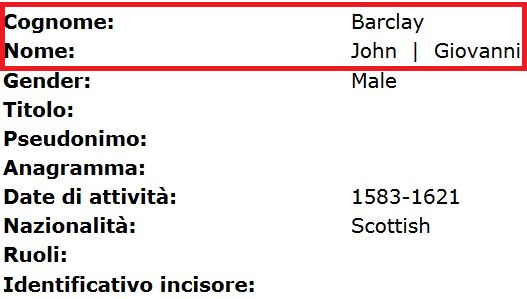
\includegraphics[width=0.6\linewidth]{database1}\\	
				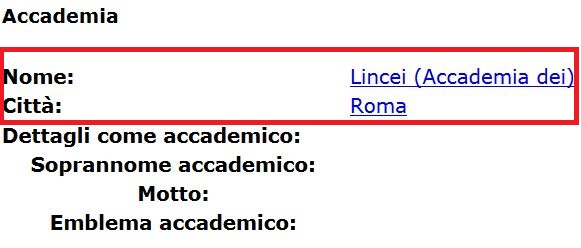
\includegraphics[width=0.6\linewidth]{database2}\\
				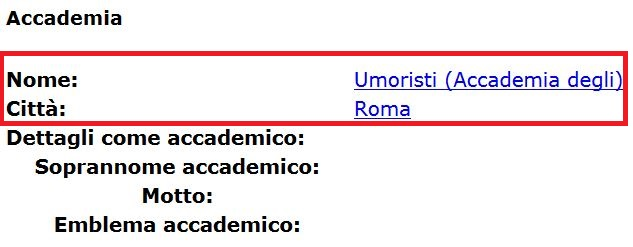
\includegraphics[width=0.6\linewidth]{database3}
			\end{figure}
		\end{column}		
		
		
	\end{columns}
	
	
	
\end{frame}
\begin{frame}
	\frametitle{Data - Censorship}
	Identify whether his (or her) work was subject to censorship by the church	
	
	\hspace{0.1cm}	
	
   \textbf{Source:} De Bujanda and Richter (2002)\vspace{0.15cm}
	\begin{itemize}
		\item Collection of Indexes of Forbidden Books
		\item Short life description to complement our data
		\item Censorship of Individual works or \textit{Opera Omnia}
	\end{itemize}
	\hspace{0.3cm}

			\begin{figure}[p]
				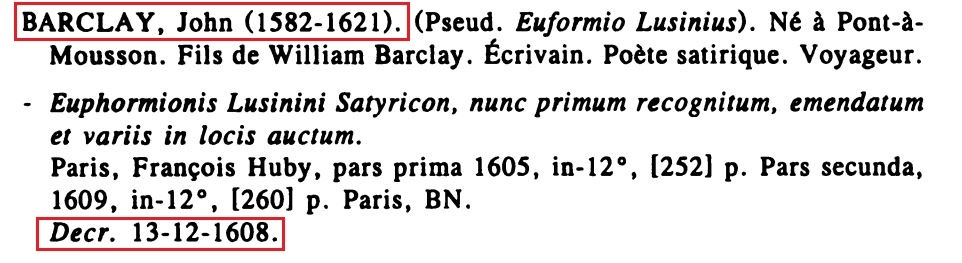
\includegraphics[width=0.75\linewidth]{librhorum}
			\end{figure}


	
\end{frame}

\begin{frame}
	\frametitle{Data - Quality of Scholars}
	We measure the “quality” of each scholar by the quantity of
	written output\vspace{0.2cm}
	
	\textbf{Source:} Worldcat search engine\vspace{0.1cm}
		\begin{itemize}
		\item References to the collections
		of thousands of libraries around the world
		\item Scholar's Quality=Log Publications by and about him
		\item Keep if at least one publication\vspace{0.1cm}
	\end{itemize}

			\begin{figure}[p]
				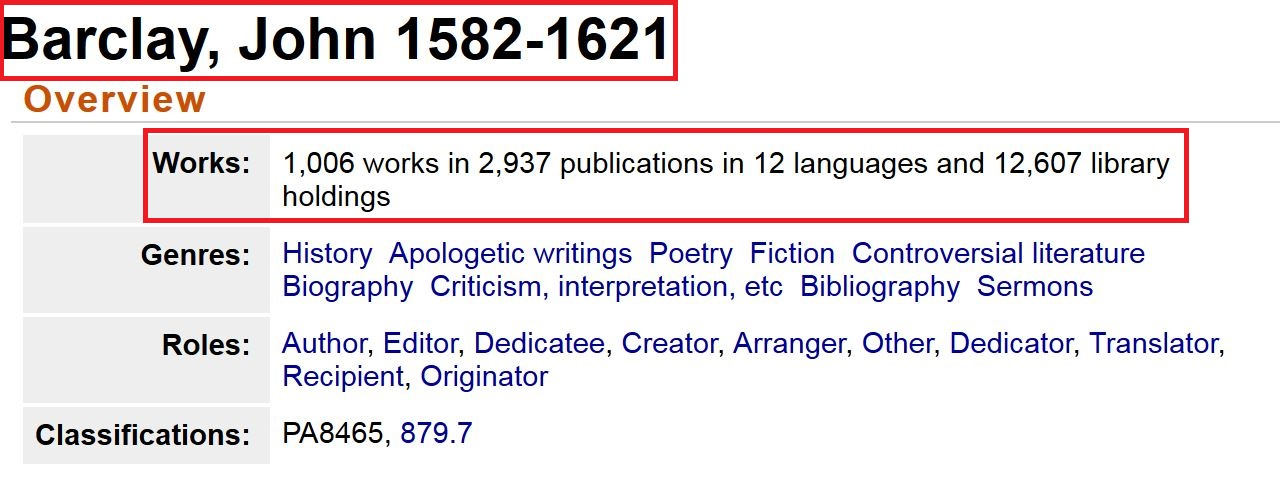
\includegraphics[width=0.62\linewidth]{worldcat}\\
			\end{figure}
		

	
\end{frame}


\begin{frame}
\frametitle{The Data in a Map - Europe}
\begin{figure}
	\centering
	\includegraphics[width=0.65\linewidth]{"C:/Users/Fabio/Dropbox/Roman_Church_censorship_growth/paper/map-europe"}
\end{figure}
\end{frame}

\begin{frame}
\frametitle{The Data in a Map - Italy }
\begin{figure}
	\includegraphics[width=0.65\linewidth]{"C:/Users/Fabio/Dropbox/Roman_Church_censorship_growth/paper/map-italy"}
\end{figure}
\end{frame}



\begin{frame}
\frametitle{Two New Features of Authors Censorship - I}
\begin{figure}[p]
	\includegraphics[width=0.35\linewidth]{"C:/Users/Fabio/Dropbox/Roman_Church_censorship_growth/paper/histo1Q"}
	\includegraphics[width=0.35\linewidth]{"C:/Users/Fabio/Dropbox/Roman_Church_censorship_growth/paper/histo2Q"}
\end{figure}


\end{frame}


\begin{frame}
	\frametitle{Two New Features of Authors Censorship - II}
	\begin{figure}[p]
		\includegraphics[width=0.35\linewidth]{"C:/Users/Fabio/Dropbox/Roman_Church_censorship_growth/paper/histo3Q"}
		\includegraphics[width=0.35\linewidth]{"C:/Users/Fabio/Dropbox/Roman_Church_censorship_growth/paper/histo4Q"}
		\includegraphics[width=0.35\linewidth]{"C:/Users/Fabio/Dropbox/Roman_Church_censorship_growth/paper/histo5Q"}
	\end{figure}
	
	
\end{frame}


\section{Theory}
 \begin{frame}{}
	\centering \Huge
	{\color{structure}\textbf{Theory}}
\end{frame}



\begin{frame}
	\frametitle{Theory}
	\begin{itemize}
		\item Discrete time\\ \vspace{0.3cm}
		\item one generation of $N$ authors alive at time\\ \vspace{0.3cm}
		\item Knowledge is embodied in books, transmitted to the next generation\\ \vspace{0.3cm}
		\item Agents learn from $\mu$ books during their life time\\ \vspace{0.3cm}
		\item Books can be \textbf{revolutionary} (R) or \textbf{compliant} (C)\vspace{0.3cm}
	  
\tikzset{every picture/.style={line width=0.75pt}} %set default line width to 0.75pt        

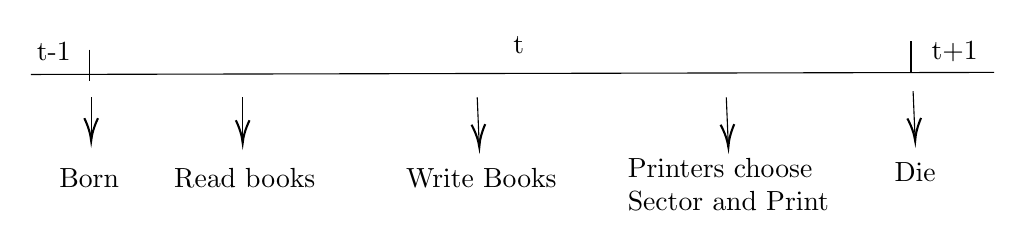
\begin{tikzpicture}[x=0.75pt,y=0.75pt,yscale=-1,xscale=1]
%uncomment if require: \path (0,300); %set diagram left start at 0, and has height of 300

%Straight Lines [id:da5177605927758191] 
\draw    (97,157) -- (561,156) ;


%Straight Lines [id:da7766036828026136] 
\draw    (125,145) -- (125,160) ;


%Straight Lines [id:da30952415765214525] 
\draw    (521,141) -- (521,156) ;


%Straight Lines [id:da9220773281159994] 
\draw    (126,168) -- (126,187) ;
\draw [shift={(126,189)}, rotate = 270] [color={rgb, 255:red, 0; green, 0; blue, 0 }  ][line width=0.75]    (10.93,-3.29) .. controls (6.95,-1.4) and (3.31,-0.3) .. (0,0) .. controls (3.31,0.3) and (6.95,1.4) .. (10.93,3.29)   ;

%Straight Lines [id:da5561040436855254] 
\draw    (199,168) -- (199,188) ;
\draw [shift={(199,190)}, rotate = 270] [color={rgb, 255:red, 0; green, 0; blue, 0 }  ][line width=0.75]    (10.93,-3.29) .. controls (6.95,-1.4) and (3.31,-0.3) .. (0,0) .. controls (3.31,0.3) and (6.95,1.4) .. (10.93,3.29)   ;

%Straight Lines [id:da35307238440341004] 
\draw    (312,168) -- (312.42,178.02) -- (312.92,190) ;
\draw [shift={(313,192)}, rotate = 267.61] [color={rgb, 255:red, 0; green, 0; blue, 0 }  ][line width=0.75]    (10.93,-3.29) .. controls (6.95,-1.4) and (3.31,-0.3) .. (0,0) .. controls (3.31,0.3) and (6.95,1.4) .. (10.93,3.29)   ;

%Straight Lines [id:da11455890173902927] 
\draw    (522,165) -- (522.92,187) ;
\draw [shift={(523,189)}, rotate = 267.61] [color={rgb, 255:red, 0; green, 0; blue, 0 }  ][line width=0.75]    (10.93,-3.29) .. controls (6.95,-1.4) and (3.31,-0.3) .. (0,0) .. controls (3.31,0.3) and (6.95,1.4) .. (10.93,3.29)   ;

%Straight Lines [id:da21202320532813468] 
\draw    (432,168) -- (432.92,190) ;
\draw [shift={(433,192)}, rotate = 267.61] [color={rgb, 255:red, 0; green, 0; blue, 0 }  ][line width=0.75]    (10.93,-3.29) .. controls (6.95,-1.4) and (3.31,-0.3) .. (0,0) .. controls (3.31,0.3) and (6.95,1.4) .. (10.93,3.29)   ;


% Text Node
\draw (108,146) node  [align=left] {t-1};
% Text Node
\draw (542,146) node  [align=left] {t+1};
% Text Node
\draw (332,143) node  [align=left] {t};
% Text Node
\draw (125,207) node  [align=left] {Born};
% Text Node
\draw (523,204) node  [align=left] {Die};
% Text Node
\draw (200,207) node  [align=left] {Read books};
% Text Node
\draw (314,207) node  [align=left] {Write Books};
% Text Node
\draw (433,210) node  [align=left] {Printers choose\\Sector and Print};


\end{tikzpicture}

	
		
		
	\end{itemize}
	
	
\end{frame}
\begin{frame}
	\frametitle{Knowledge production}
	\begin{itemize}
		\item Production using a book with irrelevance $h_i$ is $q_i$.
		\[
		q^j_i=(h^j_i)^{-\theta}, \;\;\; \theta\in(0,1),j\in\{C,R\}
		\]
		\item In $t$, the \textbf{irrelevance} of book $i$ of type $j$ follows an exponential distribution
		\[
		h^j_i \sim \exp(k^j), \quad \text{with} \ j\in \{C,R\} \ \text{and} \ i\in \{1,..,N\}.
		\]
		\item The distribution of book quality follows a Fr\'echet distribution with scale parameter $k^\theta$ and shape parameter $1/\theta$
		\item Average book quality $\bar{q}^j$ by sector j:
		\[
		E(q^j_i)=\int_0^\infty h^{-\theta}_i (k^j e^{-k^j h_i})dh_i=(k^j)^{\theta}\Gamma(1-\theta)
		\]
		
	\end{itemize}
	
\end{frame}

\begin{frame}
	\frametitle{Knowledge Accumulation}
	$m_{t-1}$ is the \textbf{share} of \textbf{revolutionary books} that people read: depends on books printed in $t-1$\vspace{0.2cm}
	
	Since exp() satisfies the minimum stability postulate, the best books retained are again exp()
	\begin{align*}	
	\hat{h}^C_i&=\text{min}\{h^C_1,..,h^C_{\lfloor(1-m_{t-1}) \mu\rfloor}\}\sim \exp(k^C_{t-1} (1-m_{t-1})\mu)=\exp(b_t^C),
	\\ \hat{h}^R_i&=\text{min}\{h^R_1,..,h^R_{\lfloor m_{t-1} \mu \rfloor}\} \sim \exp(k^R_{t-1} m_{t-1} \mu)=\exp(b_t^R)
	\end{align*}
	Combine inherited knowledge with a new idea $h^j_N\sim  \exp(\nu b^j_t)$\vspace{0.2cm}
	
	New ideas kept if more productive: knowledge evolves as
	\begin{align*}
	k_{t}^C&=(1+\nu) k_{t-1}^C (1-m_{t-1}) \mu,\\
	k_{t}^R&=(1+\nu) k_{t-1}^R m_{t-1}\mu.
	\end{align*}
	
\end{frame}

\begin{frame}
	\frametitle{Occupational Choice and Censorship}
	The Church kicks in, imposing a rate of censorship of $\beta$\\ \vspace{0.2cm}
	People will just meet $(1-\beta)\mu m_{t-1} $ revolutionary ideas\\ \vspace{0.2cm}
	Over time we have
	\[k^R_{t}=(1+\nu)\mu m_{t-1} (1-\beta) k^R_{t-1}\]
	\[k^C_{t}=(1+\nu)\mu (1-m_{t-1}) k^C_{t-1}\]
	
	Printers meet one author, pick the best type $j$ and print everyone belonging to her best book type. \vspace{0.2cm}
	
	Revolutionary ideas are weighted by $\alpha$, the relative attractiveness of revolutionary books
	\[m_t=\text{Pr}\{q^C<\alpha q^R\}=\frac{b^R_t}{b^R_t+b^C_t \alpha^{-1/\theta}}\]
\end{frame}

\begin{frame}
	\frametitle{Equilibrium path}
\begin{definition}\label{definition:equilibrium}
	Given $\beta$, an equilibrium path is a sequence $\{m_t\}_{t\geq0}$, describing the share of revolutionary books over time. It is such that:
	\begin{itemize}
		\item Each author of each generation write books whose quality and type is defined by the current state of knowledge.
		\item Each printer of each generation chooses her sector according to the most productive book presented by the first randomly met author.
		\item Each printer of each generation, once she chose her sector, prints all the authors she meets randomly.
		\item The probability of being exposed to revolutionary book in $t+1$ depends on the share of revolutionary titles written in $t$.
		\item The books printed in $t$ embody the stock of compliant and revolutionary knowledge available to generation $t+1$.
	\end{itemize}
\end{definition}
	
\end{frame}

\begin{frame}
	\frametitle{Dynamics with exogenous $\beta$}
Treating $\beta$ as an exogenous parameter dynamics are described by:\\ \vspace{0.3cm}
\begin{proposition}
	Given the initial condition $m_0\in[0,1)$, we have
	\begin{itemize}
		\item[i)]$\lim_{t\to\infty}m_t=0$ if $m_0<1/(2-\beta)$ (Compliant steady state),
		\item[ii)] $\lim_{t\to\infty}m_t=1$ if $m_0>1/(2-\beta)$ (Revolutionary steady state),
		\item[iii)]$\lim_{t\to\infty}m_t=m_0$ if $m_0=1/(2-\beta)$ (Unstable steady state).
	\end{itemize}
	%More in particular, with full censorship, or with $\beta=1$, the share of revolutionary ideas converges immediately to 0, unless $m_0=1$: in this case we will have $m_t=1 \ \forall \ t\geq0$.
	\label{proposition:dynex}
\end{proposition}
\end{frame}

\begin{frame}
	\frametitle{Church's Rule of Thumb Behavior}
What was the Church trading off? We do not know.\\ 
 We make minimal assumptions. Lexicographic preferences over:\vspace{0.3cm}
 
 \begin{enumerate}
 	\item Convergence to 0 of $m_t$\\ \vspace{0.1cm}
 	\item Minimize $\beta_t$ \\ \vspace{0.3cm}
 \end{enumerate}

\begin{proposition}
	Given the initial condition $m_0 \in [0,1)$, the Church will choose a level of censorship $\beta_t$ such that $\beta_t=\max\{2-1/m_t+\epsilon,0\}$, with $\epsilon$ arbitrarily small. If $m_0=1$, it does not exist a rate of censorship $\beta_t \in [0,1]$ such that $\lim m_t=0$.
	\label{proposition:rthumb}
\end{proposition}
\end{frame}

\begin{frame}
	\frametitle{Church's optimizing Behavior}
	Why did censorship kicked in so late, moving from virtually 0 to a considerable amount?\\ \vspace{0.15cm}

	We assume: 
	\begin{enumerate}
	\item Setting up the censoring institution was a fixed cost $\psi$
    \item The church can \textbf{censor up to $\bar{\beta}$}\vspace{0.3cm}
	\end{enumerate}
   $$	
    V(m_{t-1})=\max[{\color{green}V^N(m_{t-1})},{\color{red}V^C(m_{t-1})}-\psi]
  $$ 
  \vspace{-1.3cm}
    \begin{columns}	
    	\begin{column}[t]{0.44\textwidth}
    	 \begin{align*}
    	{\color{green}V^{N}(m_{t-1})}&{\color{green}=u(1-m_{t})+\delta V(m_{t})}	\\
    	{\color{green}\text{s.t.}}&{\color{green}\quad m_{t}=f(m_{t-1},0)}
    	\end{align*}
    	\end{column}   	
    	\begin{column}[t]{0.52\textwidth}
    	 \begin{align*}
    {\color{red}V^{C}(m_{t-1})}&{\color{red}=\max_{0\leq\beta_t\leq\overline{\beta}}u(1-m_{t-1})+\delta V^C(m_{t})}	\\
    	{\color{red}\text{s.t.}}&{\color{red}\quad m_{t}=f(m_{t-1},\beta_t)}
    	\end{align*}
    	\end{column} 	
    \end{columns}

$$  f(m_{t-1},\beta_t)=\frac{(1-\beta_t) m_{t-1}^2}{1-m_{t-1} ((\beta_t -2) m_{t-1}+2)}$$
\end{frame}

\begin{frame}
	\frametitle{Church's optimizing Behavior (cont.)}
	Trade off between censoring today paying $\psi$ and waiting\vspace{0.3cm}
	
	No censorship if 
	\begin{itemize}
		\item $m_t$ is too low: \textit{No need to censor}
		\item $m_t$ is too high: \textit{Too late to censor} \vspace{0.3cm}
	\end{itemize}

    Windows of censorship emerge
    	\begin{itemize}
    	\item Censorship if it can change dramatically the dynamics
    	\item Waiting one more period make censorship less attractive\vspace{0.3cm}
    \end{itemize}

   Still possible to have censorship and converge to $m_t=1$\vspace{0.3cm}
   
   
\end{frame}


\section{Estimation}

\begin{frame}{}
	\centering \Huge
	{\color{structure}\textbf{Estimation}}
\end{frame}
\begin{frame}
	\frametitle{Estimation}
	 
 Some parameters: taken from the literature + perfectly match moments\vspace{0.2cm}
 
 The rest is estimated down using the \textbf{simulated method of moments}
 \scriptsize
  \begin{table}[H]
  \centering % used for centering table
  \begin{tabular}{@{} l c c c @{}}  
  \hline\hline %inserts double horizontal lines
  \ External Parameters &  & Value & Target  \\ [0.05ex] % inserts table
    %heading
  \hline % inserts single horizontal line
  \rule{0pt}{2.5ex}
  Productivity of books  & $\theta$   & 0.18 & Variance of $q^R_1$  \\[0.15ex]
  Mean quality in 1  & $\overline{q}_1$   & 5.36 & First period quality  \\[0.15ex]
  Mean rev. quality in 1  & $\overline{q}^R_1$   & 7.67 & First period quality \\[0.15ex]
  \hline \hline
  \ Estimated Parameters &  & Value &  \\ [0.05ex] % inserts table
  \hline
  \ \%censored revolutionary books  & $\overline{\beta}$   & 0.15 & MSM  \\[0.15ex]
  TFP  & $(1+\nu)\mu$   & 1.66 & MSM  \\[0.15ex]
  Price of compliant books   & $p$   & 178.37 & MSM  \\[0.15ex]
  \hline
  \end{tabular}
  \end{table}

\end{frame}


\begin{frame}[label=fit]
	\frametitle{Model Fit}
  \begin{figure}[htp]	
  	\begin{subfigure}{.49\textwidth}
  		\centering
  		% include second image
  		\caption{Overall scholars\\quality: \textcolor{red}{median}, \textcolor{blue}{$75^{th}$ percentile}}
  		\label{sf:cdivbil}
  		\scalebox{0.35}{% Created by tikzDevice version 0.12.3.1 on 2022-09-19 21:45:14
% !TEX encoding = UTF-8 Unicode
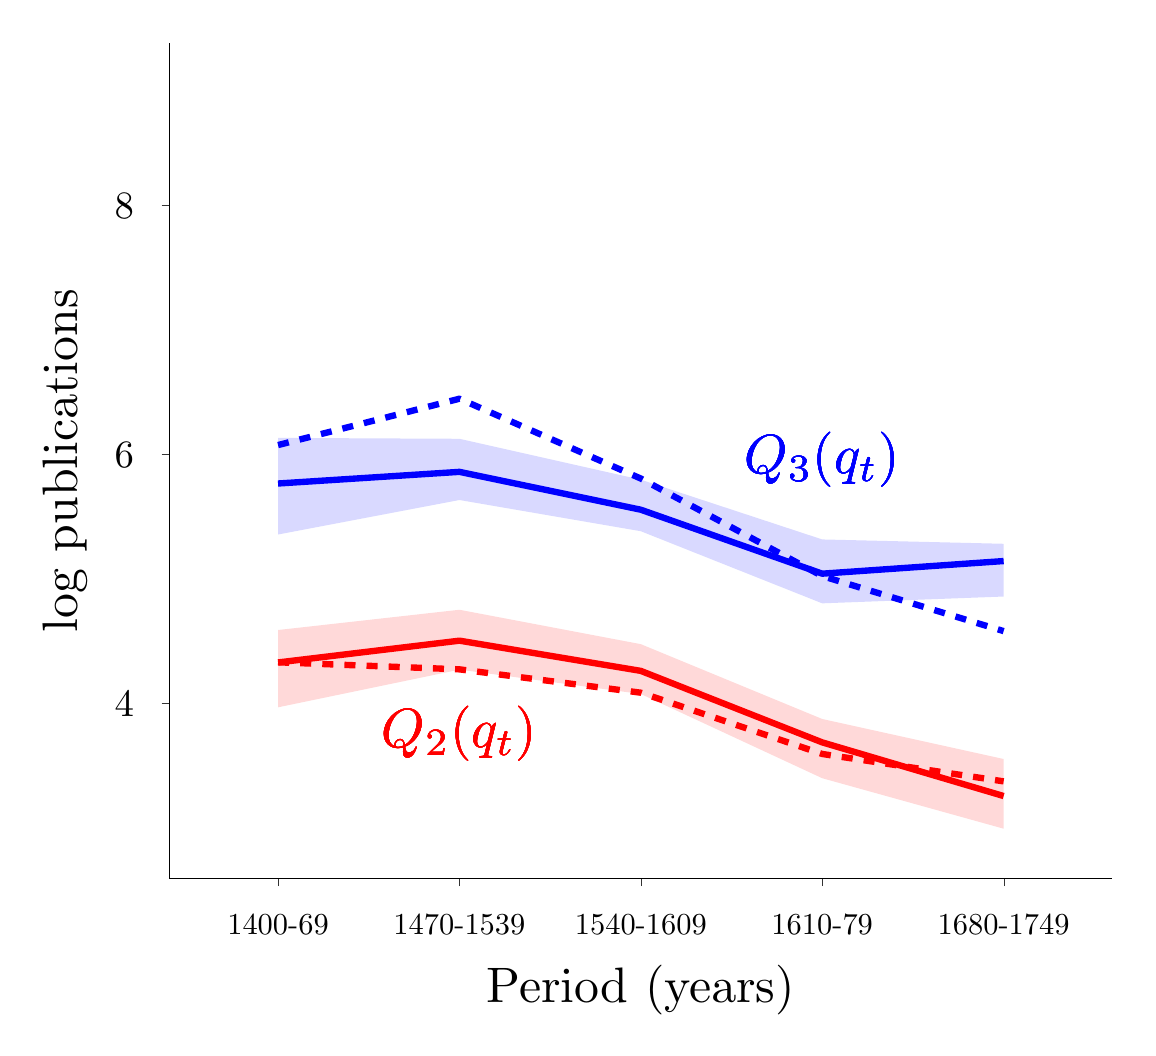
\begin{tikzpicture}[x=1pt,y=1pt]
\definecolor{fillColor}{RGB}{255,255,255}
\path[use as bounding box,fill=fillColor,fill opacity=0.00] (0,0) rectangle (397.48,361.35);
\begin{scope}
\path[clip] (  0.00,  0.00) rectangle (397.48,361.35);
\definecolor{drawColor}{RGB}{255,255,255}
\definecolor{fillColor}{RGB}{255,255,255}

\path[draw=drawColor,line width= 0.1pt,line join=round,line cap=round,fill=fillColor] (  0.00,  0.00) rectangle (397.48,361.35);
\end{scope}
\begin{scope}
\path[clip] ( 51.14, 53.86) rectangle (391.98,355.85);
\definecolor{fillColor}{RGB}{255,255,255}

\path[fill=fillColor] ( 51.14, 53.86) rectangle (391.98,355.85);
\definecolor{fillColor}{RGB}{255,0,0}

\path[fill=fillColor,fill opacity=0.15] ( 90.47,143.69) --
	(156.02,151.01) --
	(221.56,138.58) --
	(287.11,111.54) --
	(352.66, 97.08) --
	(352.66, 71.90) --
	(287.11, 90.14) --
	(221.56,120.58) --
	(156.02,129.37) --
	( 90.47,115.76) --
	cycle;

\path[] ( 90.47,143.69) --
	(156.02,151.01) --
	(221.56,138.58) --
	(287.11,111.54) --
	(352.66, 97.08);

\path[] (352.66, 71.90) --
	(287.11, 90.14) --
	(221.56,120.58) --
	(156.02,129.37) --
	( 90.47,115.76);
\definecolor{drawColor}{RGB}{255,0,0}

\path[draw=drawColor,line width= 2.3pt,line join=round] ( 90.47,131.97) --
	(156.02,139.84) --
	(221.56,128.92) --
	(287.11,103.09) --
	(352.66, 83.70);

\path[draw=drawColor,line width= 2.3pt,dash pattern=on 4pt off 4pt ,line join=round] ( 90.47,132.03) --
	(156.02,129.48) --
	(221.56,121.04) --
	(287.11, 98.90) --
	(352.66, 89.00);
\definecolor{fillColor}{RGB}{0,0,255}

\path[fill=fillColor,fill opacity=0.15] ( 90.47,213.11) --
	(156.02,212.79) --
	(221.56,198.01) --
	(287.11,176.42) --
	(352.66,174.85) --
	(352.66,155.79) --
	(287.11,153.33) --
	(221.56,179.39) --
	(156.02,190.67) --
	( 90.47,178.20) --
	cycle;

\path[] ( 90.47,213.11) --
	(156.02,212.79) --
	(221.56,198.01) --
	(287.11,176.42) --
	(352.66,174.85);

\path[] (352.66,155.79) --
	(287.11,153.33) --
	(221.56,179.39) --
	(156.02,190.67) --
	( 90.47,178.20);
\definecolor{drawColor}{RGB}{0,0,255}

\path[draw=drawColor,line width= 2.3pt,line join=round] ( 90.47,196.63) --
	(156.02,200.84) --
	(221.56,187.16) --
	(287.11,164.05) --
	(352.66,168.61);

\path[draw=drawColor,line width= 2.3pt,dash pattern=on 4pt off 4pt ,line join=round] ( 90.47,210.52) --
	(156.02,227.27) --
	(221.56,198.42) --
	(287.11,163.18) --
	(352.66,143.30);

\node[text=drawColor,anchor=base,inner sep=0pt, outer sep=0pt, scale=  1.99] at (287.11,200.25) {$Q_3(q_t)$};

\node[text=drawColor,anchor=base,inner sep=0pt, outer sep=0pt, scale=  1.99] at (287.11,200.25) {$Q_3(q_t)$};

\node[text=drawColor,anchor=base,inner sep=0pt, outer sep=0pt, scale=  1.99] at (287.11,200.25) {$Q_3(q_t)$};

\node[text=drawColor,anchor=base,inner sep=0pt, outer sep=0pt, scale=  1.99] at (287.11,200.25) {$Q_3(q_t)$};

\node[text=drawColor,anchor=base,inner sep=0pt, outer sep=0pt, scale=  1.99] at (287.11,200.25) {$Q_3(q_t)$};
\definecolor{drawColor}{RGB}{255,0,0}

\node[text=drawColor,anchor=base,inner sep=0pt, outer sep=0pt, scale=  1.99] at (156.02,101.23) {$Q_2(q_t)$};

\node[text=drawColor,anchor=base,inner sep=0pt, outer sep=0pt, scale=  1.99] at (156.02,101.23) {$Q_2(q_t)$};

\node[text=drawColor,anchor=base,inner sep=0pt, outer sep=0pt, scale=  1.99] at (156.02,101.23) {$Q_2(q_t)$};

\node[text=drawColor,anchor=base,inner sep=0pt, outer sep=0pt, scale=  1.99] at (156.02,101.23) {$Q_2(q_t)$};

\node[text=drawColor,anchor=base,inner sep=0pt, outer sep=0pt, scale=  1.99] at (156.02,101.23) {$Q_2(q_t)$};
\end{scope}
\begin{scope}
\path[clip] (  0.00,  0.00) rectangle (397.48,361.35);
\definecolor{drawColor}{RGB}{0,0,0}

\path[draw=drawColor,line width= 0.1pt,line join=round] ( 51.14, 53.86) --
	( 51.14,355.85);
\end{scope}
\begin{scope}
\path[clip] (  0.00,  0.00) rectangle (397.48,361.35);
\definecolor{drawColor}{RGB}{0,0,0}

\node[text=drawColor,anchor=base east,inner sep=0pt, outer sep=0pt, scale=  1.40] at ( 38.39,112.27) {4};

\node[text=drawColor,anchor=base east,inner sep=0pt, outer sep=0pt, scale=  1.40] at ( 38.39,202.28) {6};

\node[text=drawColor,anchor=base east,inner sep=0pt, outer sep=0pt, scale=  1.40] at ( 38.39,292.30) {8};
\end{scope}
\begin{scope}
\path[clip] (  0.00,  0.00) rectangle (397.48,361.35);
\definecolor{drawColor}{gray}{0.20}

\path[draw=drawColor,line width= 0.1pt,line join=round] ( 48.39,117.09) --
	( 51.14,117.09);

\path[draw=drawColor,line width= 0.1pt,line join=round] ( 48.39,207.11) --
	( 51.14,207.11);

\path[draw=drawColor,line width= 0.1pt,line join=round] ( 48.39,297.12) --
	( 51.14,297.12);
\end{scope}
\begin{scope}
\path[clip] (  0.00,  0.00) rectangle (397.48,361.35);
\definecolor{drawColor}{RGB}{0,0,0}

\path[draw=drawColor,line width= 0.1pt,line join=round] ( 51.14, 53.86) --
	(391.98, 53.86);
\end{scope}
\begin{scope}
\path[clip] (  0.00,  0.00) rectangle (397.48,361.35);
\definecolor{drawColor}{gray}{0.20}

\path[draw=drawColor,line width= 0.1pt,line join=round] ( 90.47, 51.11) --
	( 90.47, 53.86);

\path[draw=drawColor,line width= 0.1pt,line join=round] (156.02, 51.11) --
	(156.02, 53.86);

\path[draw=drawColor,line width= 0.1pt,line join=round] (221.56, 51.11) --
	(221.56, 53.86);

\path[draw=drawColor,line width= 0.1pt,line join=round] (287.11, 51.11) --
	(287.11, 53.86);

\path[draw=drawColor,line width= 0.1pt,line join=round] (352.66, 51.11) --
	(352.66, 53.86);
\end{scope}
\begin{scope}
\path[clip] (  0.00,  0.00) rectangle (397.48,361.35);
\definecolor{drawColor}{RGB}{0,0,0}

\node[text=drawColor,anchor=base,inner sep=0pt, outer sep=0pt, scale=  1.10] at ( 90.47, 33.53) {1400-69};

\node[text=drawColor,anchor=base,inner sep=0pt, outer sep=0pt, scale=  1.10] at (156.02, 33.53) {1470-1539};

\node[text=drawColor,anchor=base,inner sep=0pt, outer sep=0pt, scale=  1.10] at (221.56, 33.53) {1540-1609};

\node[text=drawColor,anchor=base,inner sep=0pt, outer sep=0pt, scale=  1.10] at (287.11, 33.53) {1610-79};

\node[text=drawColor,anchor=base,inner sep=0pt, outer sep=0pt, scale=  1.10] at (352.66, 33.53) {1680-1749};
\end{scope}
\begin{scope}
\path[clip] (  0.00,  0.00) rectangle (397.48,361.35);
\definecolor{drawColor}{RGB}{0,0,0}

\node[text=drawColor,anchor=base,inner sep=0pt, outer sep=0pt, scale=  1.80] at (221.56,  9.00) {Period (years)};
\end{scope}
\begin{scope}
\path[clip] (  0.00,  0.00) rectangle (397.48,361.35);
\definecolor{drawColor}{RGB}{0,0,0}

\node[text=drawColor,rotate= 90.00,anchor=base,inner sep=0pt, outer sep=0pt, scale=  1.80] at ( 17.90,204.86) {log publications};
\end{scope}
\end{tikzpicture}
 }
  	\end{subfigure}
  	\begin{subfigure}{.49\textwidth}
  		\centering
  		% include second image
  		\caption{\% censored scholars\\\textcolor{white}{a}}
  		\label{sf:cdivbil2}
  		\scalebox{0.35}{% Created by tikzDevice version 0.12.3.1 on 2022-09-19 22:27:54
% !TEX encoding = UTF-8 Unicode
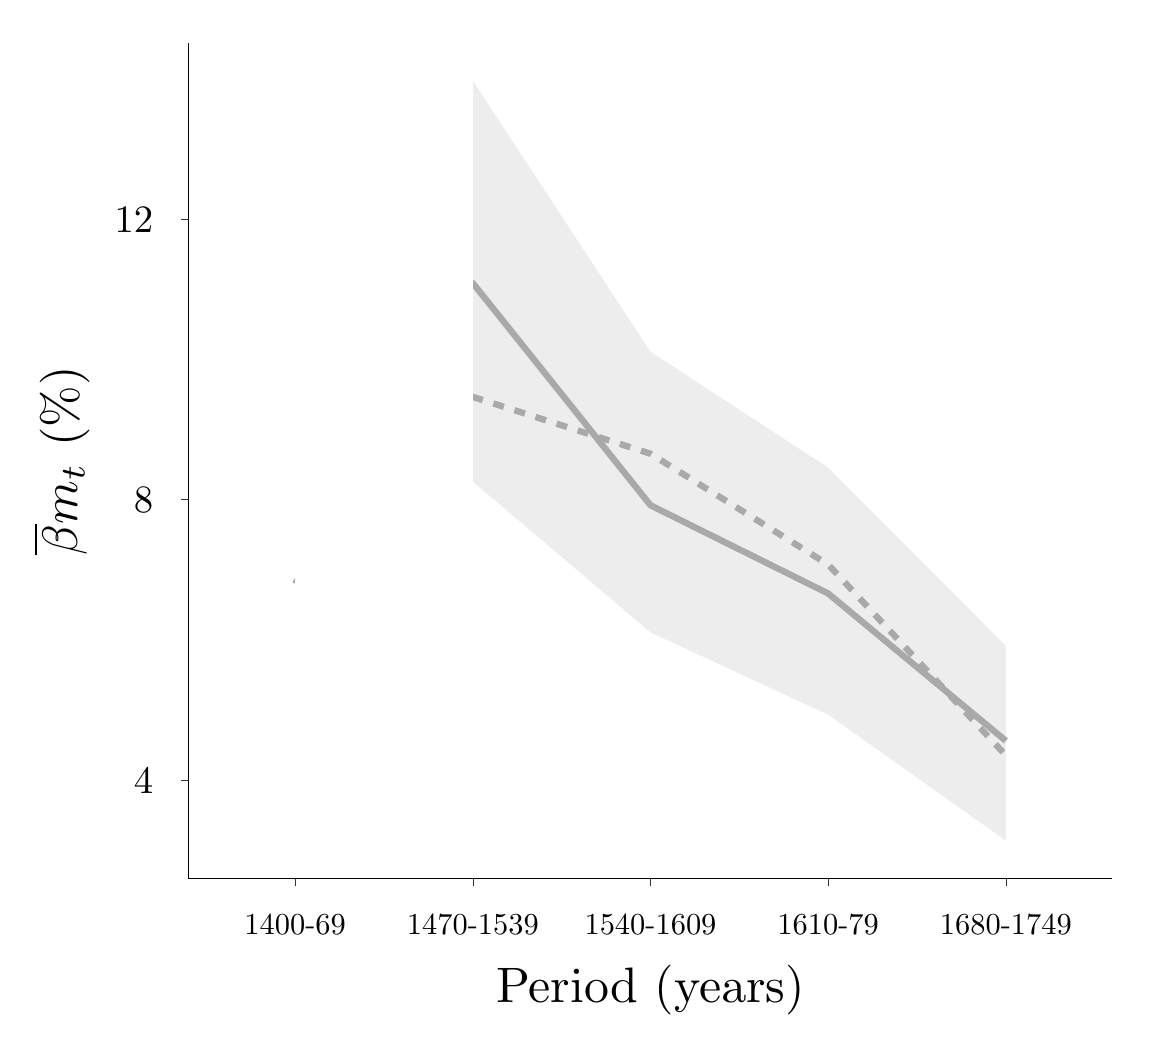
\begin{tikzpicture}[x=1pt,y=1pt]
\definecolor{fillColor}{RGB}{255,255,255}
\path[use as bounding box,fill=fillColor,fill opacity=0.00] (0,0) rectangle (397.48,361.35);
\begin{scope}
\path[clip] (  0.00,  0.00) rectangle (397.48,361.35);
\definecolor{drawColor}{RGB}{255,255,255}
\definecolor{fillColor}{RGB}{255,255,255}

\path[draw=drawColor,line width= 0.1pt,line join=round,line cap=round,fill=fillColor] (  0.00,  0.00) rectangle (397.48,361.35);
\end{scope}
\begin{scope}
\path[clip] ( 58.14, 53.86) rectangle (391.98,355.85);
\definecolor{fillColor}{RGB}{255,255,255}

\path[fill=fillColor] ( 58.14, 53.86) rectangle (391.98,355.85);
\definecolor{fillColor}{RGB}{169,169,169}

\path[fill=fillColor,fill opacity=0.20] ( 96.66,263.42) --
	(160.86,342.12) --
	(225.06,244.23) --
	(289.26,202.36) --
	(353.46,137.94) --
	(353.46, 67.59) --
	(289.26,113.10) --
	(225.06,142.83) --
	(160.86,197.32) --
	( 96.66, 75.91) --
	cycle;

\path[] ( 96.66,263.42) --
	(160.86,342.12) --
	(225.06,244.23) --
	(289.26,202.36) --
	(353.46,137.94);

\path[] (353.46, 67.59) --
	(289.26,113.10) --
	(225.06,142.83) --
	(160.86,197.32) --
	( 96.66, 75.91);
\definecolor{drawColor}{RGB}{169,169,169}

\path[draw=drawColor,line width= 2.3pt,line join=round] ( 96.66,160.39) --
	(160.86,269.05) --
	(225.06,188.77) --
	(289.26,156.89) --
	(353.46,103.64);

\path[draw=drawColor,line width= 2.3pt,dash pattern=on 4pt off 4pt ,line join=round] ( 96.66,226.06) --
	(160.86,227.93) --
	(225.06,207.39) --
	(289.26,167.35) --
	(353.46, 98.39);
\definecolor{fillColor}{RGB}{255,255,255}

\path[fill=fillColor] ( 96.66, 53.86) rectangle (160.86,355.85);

\path[fill=fillColor] ( 96.66, 53.86) rectangle (160.86,355.85);

\path[fill=fillColor] ( 96.66, 53.86) rectangle (160.86,355.85);

\path[fill=fillColor] ( 96.66, 53.86) rectangle (160.86,355.85);

\path[fill=fillColor] ( 96.66, 53.86) rectangle (160.86,355.85);
\end{scope}
\begin{scope}
\path[clip] (  0.00,  0.00) rectangle (397.48,361.35);
\definecolor{drawColor}{RGB}{0,0,0}

\path[draw=drawColor,line width= 0.1pt,line join=round] ( 58.14, 53.86) --
	( 58.14,355.85);
\end{scope}
\begin{scope}
\path[clip] (  0.00,  0.00) rectangle (397.48,361.35);
\definecolor{drawColor}{RGB}{0,0,0}

\node[text=drawColor,anchor=base east,inner sep=0pt, outer sep=0pt, scale=  1.40] at ( 45.39, 84.70) {4};

\node[text=drawColor,anchor=base east,inner sep=0pt, outer sep=0pt, scale=  1.40] at ( 45.39,186.09) {8};

\node[text=drawColor,anchor=base east,inner sep=0pt, outer sep=0pt, scale=  1.40] at ( 45.39,287.49) {12};
\end{scope}
\begin{scope}
\path[clip] (  0.00,  0.00) rectangle (397.48,361.35);
\definecolor{drawColor}{gray}{0.20}

\path[draw=drawColor,line width= 0.1pt,line join=round] ( 55.39, 89.52) --
	( 58.14, 89.52);

\path[draw=drawColor,line width= 0.1pt,line join=round] ( 55.39,190.91) --
	( 58.14,190.91);

\path[draw=drawColor,line width= 0.1pt,line join=round] ( 55.39,292.31) --
	( 58.14,292.31);
\end{scope}
\begin{scope}
\path[clip] (  0.00,  0.00) rectangle (397.48,361.35);
\definecolor{drawColor}{RGB}{0,0,0}

\path[draw=drawColor,line width= 0.1pt,line join=round] ( 58.14, 53.86) --
	(391.98, 53.86);
\end{scope}
\begin{scope}
\path[clip] (  0.00,  0.00) rectangle (397.48,361.35);
\definecolor{drawColor}{gray}{0.20}

\path[draw=drawColor,line width= 0.1pt,line join=round] ( 96.66, 51.11) --
	( 96.66, 53.86);

\path[draw=drawColor,line width= 0.1pt,line join=round] (160.86, 51.11) --
	(160.86, 53.86);

\path[draw=drawColor,line width= 0.1pt,line join=round] (225.06, 51.11) --
	(225.06, 53.86);

\path[draw=drawColor,line width= 0.1pt,line join=round] (289.26, 51.11) --
	(289.26, 53.86);

\path[draw=drawColor,line width= 0.1pt,line join=round] (353.46, 51.11) --
	(353.46, 53.86);
\end{scope}
\begin{scope}
\path[clip] (  0.00,  0.00) rectangle (397.48,361.35);
\definecolor{drawColor}{RGB}{0,0,0}

\node[text=drawColor,anchor=base,inner sep=0pt, outer sep=0pt, scale=  1.10] at ( 96.66, 33.53) {1400-69};

\node[text=drawColor,anchor=base,inner sep=0pt, outer sep=0pt, scale=  1.10] at (160.86, 33.53) {1470-1539};

\node[text=drawColor,anchor=base,inner sep=0pt, outer sep=0pt, scale=  1.10] at (225.06, 33.53) {1540-1609};

\node[text=drawColor,anchor=base,inner sep=0pt, outer sep=0pt, scale=  1.10] at (289.26, 33.53) {1610-79};

\node[text=drawColor,anchor=base,inner sep=0pt, outer sep=0pt, scale=  1.10] at (353.46, 33.53) {1680-1749};
\end{scope}
\begin{scope}
\path[clip] (  0.00,  0.00) rectangle (397.48,361.35);
\definecolor{drawColor}{RGB}{0,0,0}

\node[text=drawColor,anchor=base,inner sep=0pt, outer sep=0pt, scale=  1.80] at (225.06,  9.00) {Period (years)};
\end{scope}
\begin{scope}
\path[clip] (  0.00,  0.00) rectangle (397.48,361.35);
\definecolor{drawColor}{RGB}{0,0,0}

\node[text=drawColor,rotate= 90.00,anchor=base,inner sep=0pt, outer sep=0pt, scale=  1.80] at ( 17.90,204.86) {$\overline{\beta}m_t$ (\%)};
\end{scope}
\end{tikzpicture}
 }
  	\end{subfigure}
  \caption{Data (solid), simulations  (dashed)}

  	
  
  \end{figure}

\end{frame}


\begin{frame}
	\frametitle{Over-Identification}
	\begin{figure}
		\centering
		\begin{subfigure}{.49\textwidth}
			\centering
			% include first image
			\caption{Censored scholars\\quality: \textcolor{red}{median}, \textcolor{blue}{$75^{th}$ percentile}}
			\label{sf:cdivuni}
			\scalebox{0.35}{% Created by tikzDevice version 0.12.3.1 on 2022-09-19 22:27:53
% !TEX encoding = UTF-8 Unicode
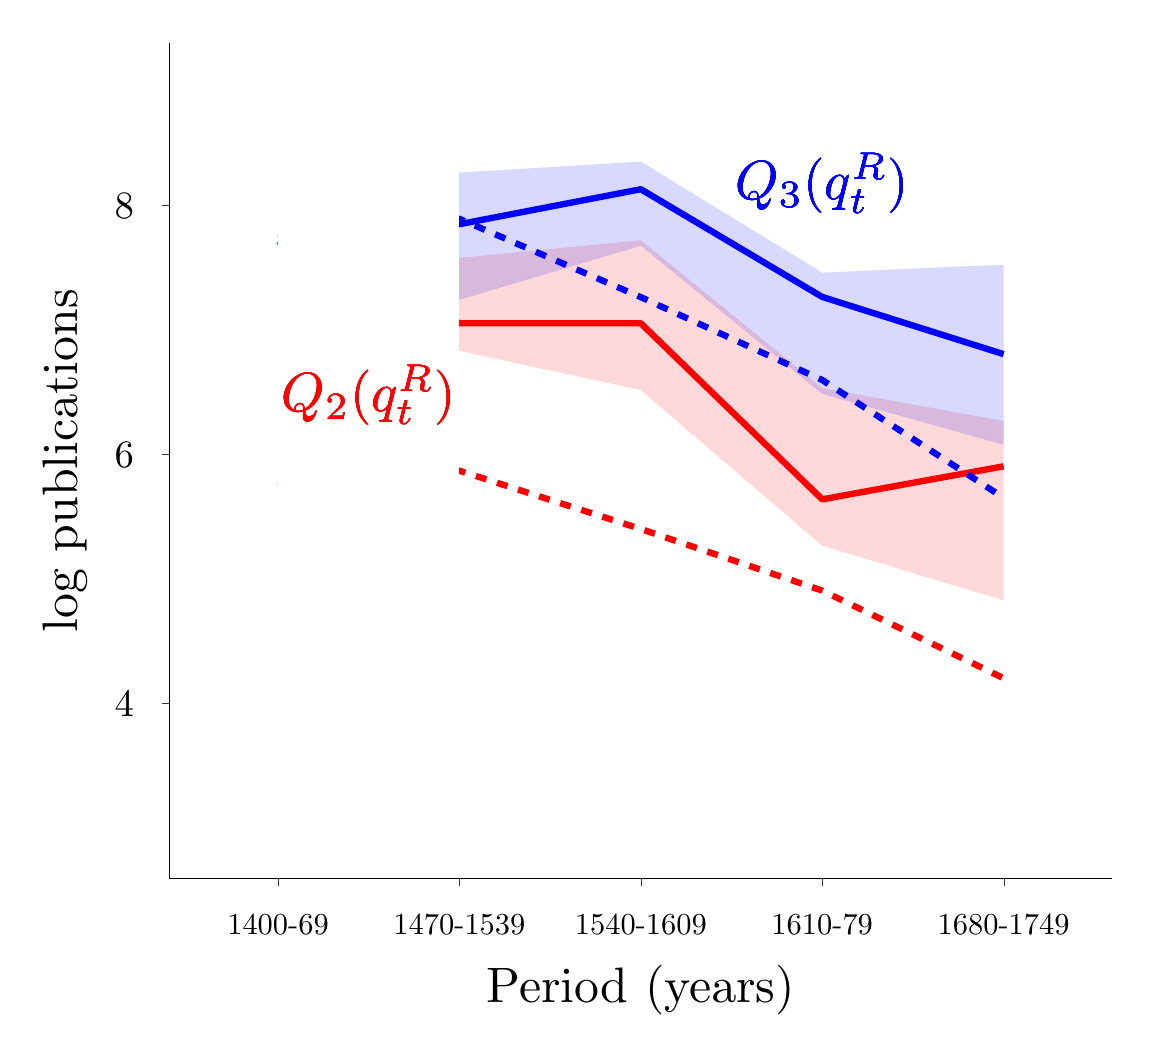
\begin{tikzpicture}[x=1pt,y=1pt]
\definecolor{fillColor}{RGB}{255,255,255}
\path[use as bounding box,fill=fillColor,fill opacity=0.00] (0,0) rectangle (397.48,361.35);
\begin{scope}
\path[clip] (  0.00,  0.00) rectangle (397.48,361.35);
\definecolor{drawColor}{RGB}{255,255,255}
\definecolor{fillColor}{RGB}{255,255,255}

\path[draw=drawColor,line width= 0.1pt,line join=round,line cap=round,fill=fillColor] (  0.00,  0.00) rectangle (397.48,361.35);
\end{scope}
\begin{scope}
\path[clip] ( 51.14, 53.86) rectangle (391.98,355.85);
\definecolor{fillColor}{RGB}{255,255,255}

\path[fill=fillColor] ( 51.14, 53.86) rectangle (391.98,355.85);
\definecolor{fillColor}{RGB}{255,0,0}

\path[fill=fillColor,fill opacity=0.15] ( 90.47,292.14) --
	(156.02,278.15) --
	(221.56,284.53) --
	(287.11,231.13) --
	(352.66,219.22) --
	(352.66,154.37) --
	(287.11,174.15) --
	(221.56,230.40) --
	(156.02,244.55) --
	( 90.47,254.76) --
	cycle;

\path[] ( 90.47,292.14) --
	(156.02,278.15) --
	(221.56,284.53) --
	(287.11,231.13) --
	(352.66,219.22);

\path[] (352.66,154.37) --
	(287.11,174.15) --
	(221.56,230.40) --
	(156.02,244.55) --
	( 90.47,254.76);
\definecolor{drawColor}{RGB}{255,0,0}

\path[draw=drawColor,line width= 2.3pt,line join=round] ( 90.47,284.23) --
	(156.02,254.56) --
	(221.56,254.52) --
	(287.11,190.91) --
	(352.66,202.85);

\path[draw=drawColor,line width= 2.3pt,dash pattern=on 4pt off 4pt ,line join=round] ( 90.47,195.87) --
	(156.02,201.25) --
	(221.56,180.20) --
	(287.11,157.93) --
	(352.66,126.27);
\definecolor{fillColor}{RGB}{0,0,255}

\path[fill=fillColor,fill opacity=0.15] ( 90.47,325.49) --
	(156.02,308.99) --
	(221.56,312.95) --
	(287.11,272.84) --
	(352.66,275.70) --
	(352.66,210.60) --
	(287.11,228.99) --
	(221.56,282.55) --
	(156.02,262.97) --
	( 90.47,278.47) --
	cycle;

\path[] ( 90.47,325.49) --
	(156.02,308.99) --
	(221.56,312.95) --
	(287.11,272.84) --
	(352.66,275.70);

\path[] (352.66,210.60) --
	(287.11,228.99) --
	(221.56,282.55) --
	(156.02,262.97) --
	( 90.47,278.47);
\definecolor{drawColor}{RGB}{0,0,255}

\path[draw=drawColor,line width= 2.3pt,line join=round] ( 90.47,291.49) --
	(156.02,290.33) --
	(221.56,302.97) --
	(287.11,264.05) --
	(352.66,243.37);

\path[draw=drawColor,line width= 2.3pt,dash pattern=on 4pt off 4pt ,line join=round] ( 90.47,285.04) --
	(156.02,292.27) --
	(221.56,263.97) --
	(287.11,234.03) --
	(352.66,191.46);
\definecolor{fillColor}{RGB}{255,255,255}

\path[fill=fillColor] ( 90.47, 53.86) rectangle (156.02,355.85);

\path[fill=fillColor] ( 90.47, 53.86) rectangle (156.02,355.85);

\path[fill=fillColor] ( 90.47, 53.86) rectangle (156.02,355.85);

\path[fill=fillColor] ( 90.47, 53.86) rectangle (156.02,355.85);

\path[fill=fillColor] ( 90.47, 53.86) rectangle (156.02,355.85);

\node[text=drawColor,anchor=base,inner sep=0pt, outer sep=0pt, scale=  1.99] at (287.11,299.26) {$Q_3(q_t^R)$};

\node[text=drawColor,anchor=base,inner sep=0pt, outer sep=0pt, scale=  1.99] at (287.11,299.26) {$Q_3(q_t^R)$};

\node[text=drawColor,anchor=base,inner sep=0pt, outer sep=0pt, scale=  1.99] at (287.11,299.26) {$Q_3(q_t^R)$};

\node[text=drawColor,anchor=base,inner sep=0pt, outer sep=0pt, scale=  1.99] at (287.11,299.26) {$Q_3(q_t^R)$};

\node[text=drawColor,anchor=base,inner sep=0pt, outer sep=0pt, scale=  1.99] at (287.11,299.26) {$Q_3(q_t^R)$};
\definecolor{drawColor}{RGB}{255,0,0}

\node[text=drawColor,anchor=base,inner sep=0pt, outer sep=0pt, scale=  1.99] at (123.25,222.75) {$Q_2(q_t^R)$};

\node[text=drawColor,anchor=base,inner sep=0pt, outer sep=0pt, scale=  1.99] at (123.25,222.75) {$Q_2(q_t^R)$};

\node[text=drawColor,anchor=base,inner sep=0pt, outer sep=0pt, scale=  1.99] at (123.25,222.75) {$Q_2(q_t^R)$};

\node[text=drawColor,anchor=base,inner sep=0pt, outer sep=0pt, scale=  1.99] at (123.25,222.75) {$Q_2(q_t^R)$};

\node[text=drawColor,anchor=base,inner sep=0pt, outer sep=0pt, scale=  1.99] at (123.25,222.75) {$Q_2(q_t^R)$};
\end{scope}
\begin{scope}
\path[clip] (  0.00,  0.00) rectangle (397.48,361.35);
\definecolor{drawColor}{RGB}{0,0,0}

\path[draw=drawColor,line width= 0.1pt,line join=round] ( 51.14, 53.86) --
	( 51.14,355.85);
\end{scope}
\begin{scope}
\path[clip] (  0.00,  0.00) rectangle (397.48,361.35);
\definecolor{drawColor}{RGB}{0,0,0}

\node[text=drawColor,anchor=base east,inner sep=0pt, outer sep=0pt, scale=  1.40] at ( 38.39,112.27) {4};

\node[text=drawColor,anchor=base east,inner sep=0pt, outer sep=0pt, scale=  1.40] at ( 38.39,202.28) {6};

\node[text=drawColor,anchor=base east,inner sep=0pt, outer sep=0pt, scale=  1.40] at ( 38.39,292.30) {8};
\end{scope}
\begin{scope}
\path[clip] (  0.00,  0.00) rectangle (397.48,361.35);
\definecolor{drawColor}{gray}{0.20}

\path[draw=drawColor,line width= 0.1pt,line join=round] ( 48.39,117.09) --
	( 51.14,117.09);

\path[draw=drawColor,line width= 0.1pt,line join=round] ( 48.39,207.11) --
	( 51.14,207.11);

\path[draw=drawColor,line width= 0.1pt,line join=round] ( 48.39,297.12) --
	( 51.14,297.12);
\end{scope}
\begin{scope}
\path[clip] (  0.00,  0.00) rectangle (397.48,361.35);
\definecolor{drawColor}{RGB}{0,0,0}

\path[draw=drawColor,line width= 0.1pt,line join=round] ( 51.14, 53.86) --
	(391.98, 53.86);
\end{scope}
\begin{scope}
\path[clip] (  0.00,  0.00) rectangle (397.48,361.35);
\definecolor{drawColor}{gray}{0.20}

\path[draw=drawColor,line width= 0.1pt,line join=round] ( 90.47, 51.11) --
	( 90.47, 53.86);

\path[draw=drawColor,line width= 0.1pt,line join=round] (156.02, 51.11) --
	(156.02, 53.86);

\path[draw=drawColor,line width= 0.1pt,line join=round] (221.56, 51.11) --
	(221.56, 53.86);

\path[draw=drawColor,line width= 0.1pt,line join=round] (287.11, 51.11) --
	(287.11, 53.86);

\path[draw=drawColor,line width= 0.1pt,line join=round] (352.66, 51.11) --
	(352.66, 53.86);
\end{scope}
\begin{scope}
\path[clip] (  0.00,  0.00) rectangle (397.48,361.35);
\definecolor{drawColor}{RGB}{0,0,0}

\node[text=drawColor,anchor=base,inner sep=0pt, outer sep=0pt, scale=  1.10] at ( 90.47, 33.53) {1400-69};

\node[text=drawColor,anchor=base,inner sep=0pt, outer sep=0pt, scale=  1.10] at (156.02, 33.53) {1470-1539};

\node[text=drawColor,anchor=base,inner sep=0pt, outer sep=0pt, scale=  1.10] at (221.56, 33.53) {1540-1609};

\node[text=drawColor,anchor=base,inner sep=0pt, outer sep=0pt, scale=  1.10] at (287.11, 33.53) {1610-79};

\node[text=drawColor,anchor=base,inner sep=0pt, outer sep=0pt, scale=  1.10] at (352.66, 33.53) {1680-1749};
\end{scope}
\begin{scope}
\path[clip] (  0.00,  0.00) rectangle (397.48,361.35);
\definecolor{drawColor}{RGB}{0,0,0}

\node[text=drawColor,anchor=base,inner sep=0pt, outer sep=0pt, scale=  1.80] at (221.56,  9.00) {Period (years)};
\end{scope}
\begin{scope}
\path[clip] (  0.00,  0.00) rectangle (397.48,361.35);
\definecolor{drawColor}{RGB}{0,0,0}

\node[text=drawColor,rotate= 90.00,anchor=base,inner sep=0pt, outer sep=0pt, scale=  1.80] at ( 17.90,204.86) {log publications};
\end{scope}
\end{tikzpicture}
 }
		\end{subfigure}
		\begin{subfigure}{.49\textwidth}
			\centering
			% include first image
			\caption{Non-censored scholars\\quality: \textcolor{red}{median}, \textcolor{blue}{$75^{th}$ percentile}}
			\label{sf:cdivuni2}
			\scalebox{0.35}{% Created by tikzDevice version 0.12.3.1 on 2022-09-19 22:27:53
% !TEX encoding = UTF-8 Unicode
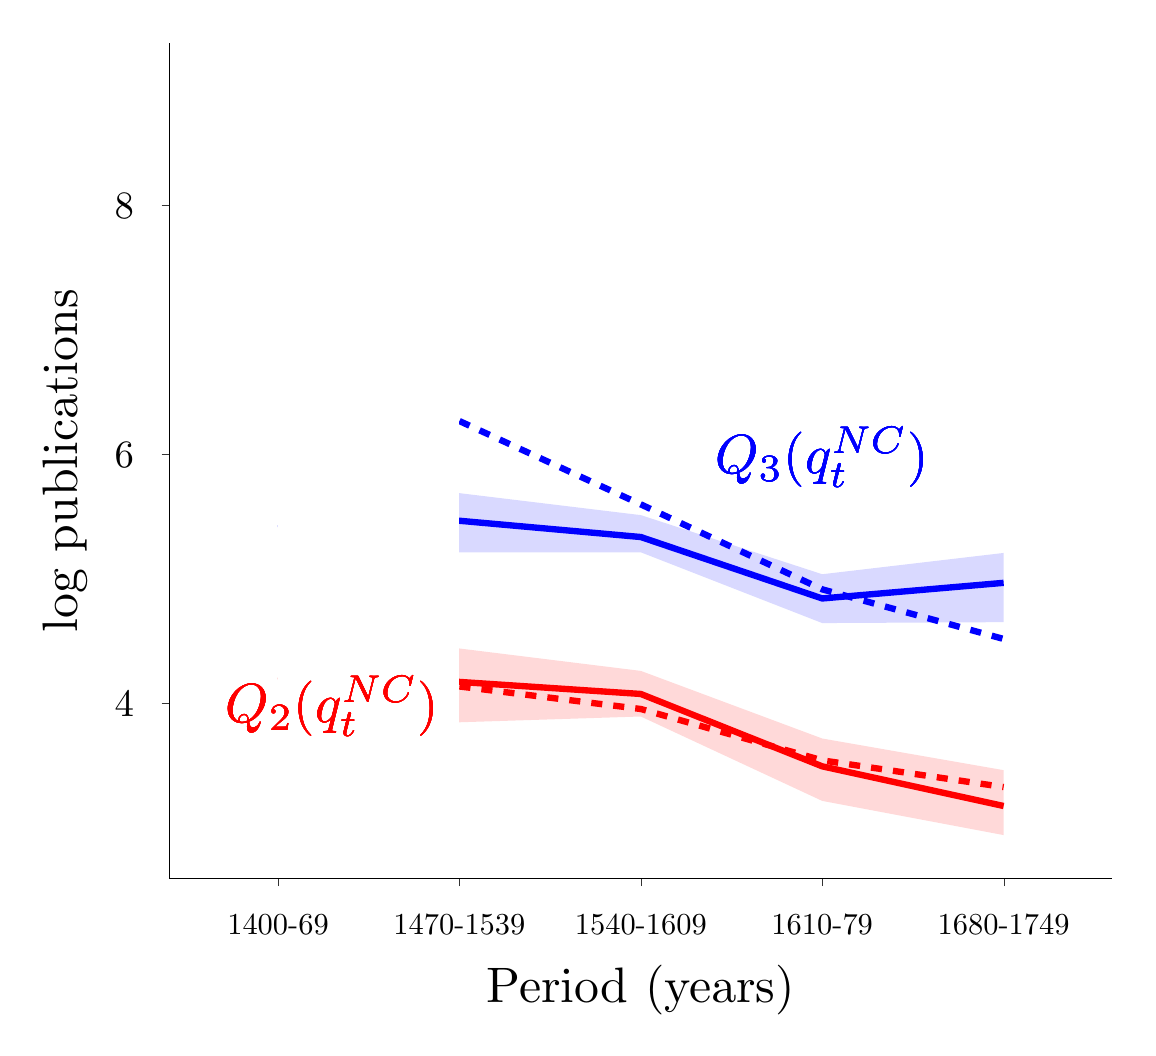
\begin{tikzpicture}[x=1pt,y=1pt]
\definecolor{fillColor}{RGB}{255,255,255}
\path[use as bounding box,fill=fillColor,fill opacity=0.00] (0,0) rectangle (397.48,361.35);
\begin{scope}
\path[clip] (  0.00,  0.00) rectangle (397.48,361.35);
\definecolor{drawColor}{RGB}{255,255,255}
\definecolor{fillColor}{RGB}{255,255,255}

\path[draw=drawColor,line width= 0.1pt,line join=round,line cap=round,fill=fillColor] (  0.00,  0.00) rectangle (397.48,361.35);
\end{scope}
\begin{scope}
\path[clip] ( 51.14, 53.86) rectangle (391.98,355.85);
\definecolor{fillColor}{RGB}{255,255,255}

\path[fill=fillColor] ( 51.14, 53.86) rectangle (391.98,355.85);
\definecolor{fillColor}{RGB}{255,0,0}

\path[fill=fillColor,fill opacity=0.15] ( 90.47,136.22) --
	(156.02,137.02) --
	(221.56,128.92) --
	(287.11,104.49) --
	(352.66, 93.05) --
	(352.66, 69.59) --
	(287.11, 81.94) --
	(221.56,112.44) --
	(156.02,110.35) --
	( 90.47,106.78) --
	cycle;

\path[] ( 90.47,136.22) --
	(156.02,137.02) --
	(221.56,128.92) --
	(287.11,104.49) --
	(352.66, 93.05);

\path[] (352.66, 69.59) --
	(287.11, 81.94) --
	(221.56,112.44) --
	(156.02,110.35) --
	( 90.47,106.78);
\definecolor{drawColor}{RGB}{255,0,0}

\path[draw=drawColor,line width= 2.3pt,line join=round] ( 90.47,126.97) --
	(156.02,124.94) --
	(221.56,120.58) --
	(287.11, 94.43) --
	(352.66, 80.10);

\path[draw=drawColor,line width= 2.3pt,dash pattern=on 4pt off 4pt ,line join=round] (156.02,123.30) --
	(221.56,115.15) --
	(287.11, 96.59) --
	(352.66, 86.95);
\definecolor{fillColor}{RGB}{0,0,255}

\path[fill=fillColor,fill opacity=0.15] ( 90.47,199.10) --
	(156.02,193.15) --
	(221.56,185.21) --
	(287.11,163.85) --
	(352.66,171.54) --
	(352.66,146.53) --
	(287.11,146.20) --
	(221.56,171.77) --
	(156.02,171.76) --
	( 90.47,164.34) --
	cycle;

\path[] ( 90.47,199.10) --
	(156.02,193.15) --
	(221.56,185.21) --
	(287.11,163.85) --
	(352.66,171.54);

\path[] (352.66,146.53) --
	(287.11,146.20) --
	(221.56,171.77) --
	(156.02,171.76) --
	( 90.47,164.34);
\definecolor{drawColor}{RGB}{0,0,255}

\path[draw=drawColor,line width= 2.3pt,line join=round] ( 90.47,180.48) --
	(156.02,183.17) --
	(221.56,177.29) --
	(287.11,155.09) --
	(352.66,160.74);

\path[draw=drawColor,line width= 2.3pt,dash pattern=on 4pt off 4pt ,line join=round] (156.02,219.20) --
	(221.56,189.09) --
	(287.11,158.39) --
	(352.66,140.46);
\definecolor{fillColor}{RGB}{255,255,255}

\path[fill=fillColor] ( 90.47, 53.86) rectangle (156.02,355.85);

\path[fill=fillColor] ( 90.47, 53.86) rectangle (156.02,355.85);

\path[fill=fillColor] ( 90.47, 53.86) rectangle (156.02,355.85);

\path[fill=fillColor] ( 90.47, 53.86) rectangle (156.02,355.85);

\path[fill=fillColor] ( 90.47, 53.86) rectangle (156.02,355.85);

\node[text=drawColor,anchor=base,inner sep=0pt, outer sep=0pt, scale=  1.99] at (287.11,200.25) {$Q_3(q_t^{NC})$};

\node[text=drawColor,anchor=base,inner sep=0pt, outer sep=0pt, scale=  1.99] at (287.11,200.25) {$Q_3(q_t^{NC})$};

\node[text=drawColor,anchor=base,inner sep=0pt, outer sep=0pt, scale=  1.99] at (287.11,200.25) {$Q_3(q_t^{NC})$};

\node[text=drawColor,anchor=base,inner sep=0pt, outer sep=0pt, scale=  1.99] at (287.11,200.25) {$Q_3(q_t^{NC})$};

\node[text=drawColor,anchor=base,inner sep=0pt, outer sep=0pt, scale=  1.99] at (287.11,200.25) {$Q_3(q_t^{NC})$};
\definecolor{drawColor}{RGB}{255,0,0}

\node[text=drawColor,anchor=base,inner sep=0pt, outer sep=0pt, scale=  1.99] at (110.14,110.23) {$Q_2(q_t^{NC})$};

\node[text=drawColor,anchor=base,inner sep=0pt, outer sep=0pt, scale=  1.99] at (110.14,110.23) {$Q_2(q_t^{NC})$};

\node[text=drawColor,anchor=base,inner sep=0pt, outer sep=0pt, scale=  1.99] at (110.14,110.23) {$Q_2(q_t^{NC})$};

\node[text=drawColor,anchor=base,inner sep=0pt, outer sep=0pt, scale=  1.99] at (110.14,110.23) {$Q_2(q_t^{NC})$};

\node[text=drawColor,anchor=base,inner sep=0pt, outer sep=0pt, scale=  1.99] at (110.14,110.23) {$Q_2(q_t^{NC})$};
\end{scope}
\begin{scope}
\path[clip] (  0.00,  0.00) rectangle (397.48,361.35);
\definecolor{drawColor}{RGB}{0,0,0}

\path[draw=drawColor,line width= 0.1pt,line join=round] ( 51.14, 53.86) --
	( 51.14,355.85);
\end{scope}
\begin{scope}
\path[clip] (  0.00,  0.00) rectangle (397.48,361.35);
\definecolor{drawColor}{RGB}{0,0,0}

\node[text=drawColor,anchor=base east,inner sep=0pt, outer sep=0pt, scale=  1.40] at ( 38.39,112.27) {4};

\node[text=drawColor,anchor=base east,inner sep=0pt, outer sep=0pt, scale=  1.40] at ( 38.39,202.28) {6};

\node[text=drawColor,anchor=base east,inner sep=0pt, outer sep=0pt, scale=  1.40] at ( 38.39,292.30) {8};
\end{scope}
\begin{scope}
\path[clip] (  0.00,  0.00) rectangle (397.48,361.35);
\definecolor{drawColor}{gray}{0.20}

\path[draw=drawColor,line width= 0.1pt,line join=round] ( 48.39,117.09) --
	( 51.14,117.09);

\path[draw=drawColor,line width= 0.1pt,line join=round] ( 48.39,207.11) --
	( 51.14,207.11);

\path[draw=drawColor,line width= 0.1pt,line join=round] ( 48.39,297.12) --
	( 51.14,297.12);
\end{scope}
\begin{scope}
\path[clip] (  0.00,  0.00) rectangle (397.48,361.35);
\definecolor{drawColor}{RGB}{0,0,0}

\path[draw=drawColor,line width= 0.1pt,line join=round] ( 51.14, 53.86) --
	(391.98, 53.86);
\end{scope}
\begin{scope}
\path[clip] (  0.00,  0.00) rectangle (397.48,361.35);
\definecolor{drawColor}{gray}{0.20}

\path[draw=drawColor,line width= 0.1pt,line join=round] ( 90.47, 51.11) --
	( 90.47, 53.86);

\path[draw=drawColor,line width= 0.1pt,line join=round] (156.02, 51.11) --
	(156.02, 53.86);

\path[draw=drawColor,line width= 0.1pt,line join=round] (221.56, 51.11) --
	(221.56, 53.86);

\path[draw=drawColor,line width= 0.1pt,line join=round] (287.11, 51.11) --
	(287.11, 53.86);

\path[draw=drawColor,line width= 0.1pt,line join=round] (352.66, 51.11) --
	(352.66, 53.86);
\end{scope}
\begin{scope}
\path[clip] (  0.00,  0.00) rectangle (397.48,361.35);
\definecolor{drawColor}{RGB}{0,0,0}

\node[text=drawColor,anchor=base,inner sep=0pt, outer sep=0pt, scale=  1.10] at ( 90.47, 33.53) {1400-69};

\node[text=drawColor,anchor=base,inner sep=0pt, outer sep=0pt, scale=  1.10] at (156.02, 33.53) {1470-1539};

\node[text=drawColor,anchor=base,inner sep=0pt, outer sep=0pt, scale=  1.10] at (221.56, 33.53) {1540-1609};

\node[text=drawColor,anchor=base,inner sep=0pt, outer sep=0pt, scale=  1.10] at (287.11, 33.53) {1610-79};

\node[text=drawColor,anchor=base,inner sep=0pt, outer sep=0pt, scale=  1.10] at (352.66, 33.53) {1680-1749};
\end{scope}
\begin{scope}
\path[clip] (  0.00,  0.00) rectangle (397.48,361.35);
\definecolor{drawColor}{RGB}{0,0,0}

\node[text=drawColor,anchor=base,inner sep=0pt, outer sep=0pt, scale=  1.80] at (221.56,  9.00) {Period (years)};
\end{scope}
\begin{scope}
\path[clip] (  0.00,  0.00) rectangle (397.48,361.35);
\definecolor{drawColor}{RGB}{0,0,0}

\node[text=drawColor,rotate= 90.00,anchor=base,inner sep=0pt, outer sep=0pt, scale=  1.80] at ( 17.90,204.86) {log publications};
\end{scope}
\end{tikzpicture}
 }
		\end{subfigure}
	\caption{Data (solid), simulations  (dashed)}
	\end{figure}
	
\end{frame}



\section{Counterfactual Experiment}

\begin{frame}{}
	\centering \Huge
	{\color{structure}\textbf{Counterfactual Experiments}}
\end{frame}

\begin{frame}
	\frametitle{Counterfactual Dynamics without Censorship}
  \begin{figure}[htbp]	
  	\centering
  	\hspace*{-1cm}
  	\begin{subfigure}{.32\textwidth}
  		\centering
  		% include second image
  		\caption{\% censored authors\\\textcolor{white}{a}\\\textcolor{white}{a}}
  		\label{sf:ca}
  		\scalebox{0.35}{% Created by tikzDevice version 0.12.3.1 on 2022-09-19 21:45:17
% !TEX encoding = UTF-8 Unicode
\begin{tikzpicture}[x=1pt,y=1pt]
\definecolor{fillColor}{RGB}{255,255,255}
\path[use as bounding box,fill=fillColor,fill opacity=0.00] (0,0) rectangle (397.48,289.08);
\begin{scope}
\path[clip] (  0.00,  0.00) rectangle (397.48,289.08);
\definecolor{drawColor}{RGB}{255,255,255}
\definecolor{fillColor}{RGB}{255,255,255}

\path[draw=drawColor,line width= 0.1pt,line join=round,line cap=round,fill=fillColor] (  0.00,  0.00) rectangle (397.48,289.08);
\end{scope}
\begin{scope}
\path[clip] ( 51.14, 53.86) rectangle (391.98,283.58);
\definecolor{fillColor}{RGB}{255,255,255}

\path[fill=fillColor] ( 51.14, 53.86) rectangle (391.98,283.58);
\definecolor{drawColor}{RGB}{169,169,169}

\path[draw=drawColor,line width= 2.3pt,line join=round] ( 90.47,271.50) --
	(156.02,273.14) --
	(221.56,255.25) --
	(287.11,220.38) --
	(352.66,160.32);

\path[draw=drawColor,line width= 2.3pt,dash pattern=on 4pt off 4pt ,line join=round] ( 90.47, 64.30) --
	(156.02, 64.30) --
	(221.56, 64.30) --
	(287.11, 64.30) --
	(352.66, 64.30);

\path[fill=fillColor] ( 90.47, 53.86) rectangle (156.02,283.58);

\path[fill=fillColor] ( 90.47, 53.86) rectangle (156.02,283.58);

\path[fill=fillColor] ( 90.47, 53.86) rectangle (156.02,283.58);

\path[fill=fillColor] ( 90.47, 53.86) rectangle (156.02,283.58);

\path[fill=fillColor] ( 90.47, 53.86) rectangle (156.02,283.58);
\end{scope}
\begin{scope}
\path[clip] (  0.00,  0.00) rectangle (397.48,289.08);
\definecolor{drawColor}{RGB}{0,0,0}

\path[draw=drawColor,line width= 0.1pt,line join=round] ( 51.14, 53.86) --
	( 51.14,283.58);
\end{scope}
\begin{scope}
\path[clip] (  0.00,  0.00) rectangle (397.48,289.08);
\definecolor{drawColor}{RGB}{0,0,0}

\node[text=drawColor,anchor=base east,inner sep=0pt, outer sep=0pt, scale=  1.40] at ( 38.39,147.78) {4};

\node[text=drawColor,anchor=base east,inner sep=0pt, outer sep=0pt, scale=  1.40] at ( 38.39,236.08) {8};
\end{scope}
\begin{scope}
\path[clip] (  0.00,  0.00) rectangle (397.48,289.08);
\definecolor{drawColor}{gray}{0.20}

\path[draw=drawColor,line width= 0.1pt,line join=round] ( 48.39,152.60) --
	( 51.14,152.60);

\path[draw=drawColor,line width= 0.1pt,line join=round] ( 48.39,240.90) --
	( 51.14,240.90);
\end{scope}
\begin{scope}
\path[clip] (  0.00,  0.00) rectangle (397.48,289.08);
\definecolor{drawColor}{RGB}{0,0,0}

\path[draw=drawColor,line width= 0.1pt,line join=round] ( 51.14, 53.86) --
	(391.98, 53.86);
\end{scope}
\begin{scope}
\path[clip] (  0.00,  0.00) rectangle (397.48,289.08);
\definecolor{drawColor}{gray}{0.20}

\path[draw=drawColor,line width= 0.1pt,line join=round] ( 90.47, 51.11) --
	( 90.47, 53.86);

\path[draw=drawColor,line width= 0.1pt,line join=round] (156.02, 51.11) --
	(156.02, 53.86);

\path[draw=drawColor,line width= 0.1pt,line join=round] (221.56, 51.11) --
	(221.56, 53.86);

\path[draw=drawColor,line width= 0.1pt,line join=round] (287.11, 51.11) --
	(287.11, 53.86);

\path[draw=drawColor,line width= 0.1pt,line join=round] (352.66, 51.11) --
	(352.66, 53.86);
\end{scope}
\begin{scope}
\path[clip] (  0.00,  0.00) rectangle (397.48,289.08);
\definecolor{drawColor}{RGB}{0,0,0}

\node[text=drawColor,anchor=base,inner sep=0pt, outer sep=0pt, scale=  1.10] at ( 90.47, 33.53) {1400-69};

\node[text=drawColor,anchor=base,inner sep=0pt, outer sep=0pt, scale=  1.10] at (156.02, 33.53) {1470-1539};

\node[text=drawColor,anchor=base,inner sep=0pt, outer sep=0pt, scale=  1.10] at (221.56, 33.53) {1540-1609};

\node[text=drawColor,anchor=base,inner sep=0pt, outer sep=0pt, scale=  1.10] at (287.11, 33.53) {1610-79};

\node[text=drawColor,anchor=base,inner sep=0pt, outer sep=0pt, scale=  1.10] at (352.66, 33.53) {1680-1749};
\end{scope}
\begin{scope}
\path[clip] (  0.00,  0.00) rectangle (397.48,289.08);
\definecolor{drawColor}{RGB}{0,0,0}

\node[text=drawColor,anchor=base,inner sep=0pt, outer sep=0pt, scale=  1.80] at (221.56,  9.00) {Period (years)};
\end{scope}
\begin{scope}
\path[clip] (  0.00,  0.00) rectangle (397.48,289.08);
\definecolor{drawColor}{RGB}{0,0,0}

\node[text=drawColor,rotate= 90.00,anchor=base,inner sep=0pt, outer sep=0pt, scale=  1.80] at ( 17.90,168.72) {$\overline{\beta}m_t$ (\%) };
\end{scope}
\end{tikzpicture}
 }
  	\end{subfigure}
  	\begin{subfigure}{.32\textwidth}
  		\centering
  		% include first image
  		\caption{\% revolutionary authors\\\textcolor{white}{a}}
  		\label{sf:ra}
  		\scalebox{0.35}{% Created by tikzDevice version 0.12.3.1 on 2022-09-19 22:27:55
% !TEX encoding = UTF-8 Unicode
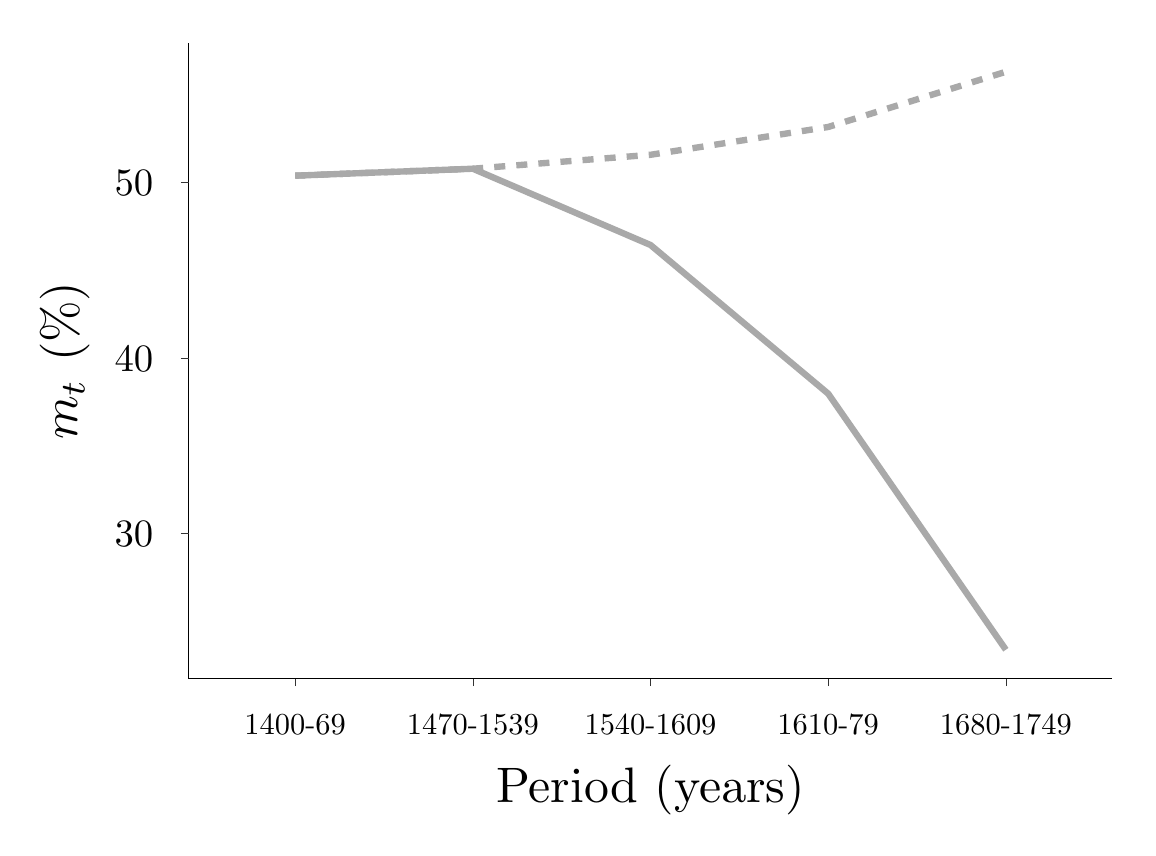
\begin{tikzpicture}[x=1pt,y=1pt]
\definecolor{fillColor}{RGB}{255,255,255}
\path[use as bounding box,fill=fillColor,fill opacity=0.00] (0,0) rectangle (397.48,289.08);
\begin{scope}
\path[clip] (  0.00,  0.00) rectangle (397.48,289.08);
\definecolor{drawColor}{RGB}{255,255,255}
\definecolor{fillColor}{RGB}{255,255,255}

\path[draw=drawColor,line width= 0.1pt,line join=round,line cap=round,fill=fillColor] (  0.00,  0.00) rectangle (397.48,289.08);
\end{scope}
\begin{scope}
\path[clip] ( 58.14, 53.86) rectangle (391.98,283.58);
\definecolor{fillColor}{RGB}{255,255,255}

\path[fill=fillColor] ( 58.14, 53.86) rectangle (391.98,283.58);
\definecolor{drawColor}{RGB}{169,169,169}

\path[draw=drawColor,line width= 2.3pt,line join=round] ( 96.66,235.59) --
	(160.86,238.11) --
	(225.06,210.55) --
	(289.26,156.83) --
	(353.46, 64.30);

\path[draw=drawColor,line width= 2.3pt,dash pattern=on 4pt off 4pt ,line join=round] ( 96.66,235.59) --
	(160.86,238.11) --
	(225.06,243.14) --
	(289.26,253.19) --
	(353.46,273.14);
\end{scope}
\begin{scope}
\path[clip] (  0.00,  0.00) rectangle (397.48,289.08);
\definecolor{drawColor}{RGB}{0,0,0}

\path[draw=drawColor,line width= 0.1pt,line join=round] ( 58.14, 53.86) --
	( 58.14,283.58);
\end{scope}
\begin{scope}
\path[clip] (  0.00,  0.00) rectangle (397.48,289.08);
\definecolor{drawColor}{RGB}{0,0,0}

\node[text=drawColor,anchor=base east,inner sep=0pt, outer sep=0pt, scale=  1.40] at ( 45.39,101.57) {30};

\node[text=drawColor,anchor=base east,inner sep=0pt, outer sep=0pt, scale=  1.40] at ( 45.39,164.91) {40};

\node[text=drawColor,anchor=base east,inner sep=0pt, outer sep=0pt, scale=  1.40] at ( 45.39,228.26) {50};
\end{scope}
\begin{scope}
\path[clip] (  0.00,  0.00) rectangle (397.48,289.08);
\definecolor{drawColor}{gray}{0.20}

\path[draw=drawColor,line width= 0.1pt,line join=round] ( 55.39,106.39) --
	( 58.14,106.39);

\path[draw=drawColor,line width= 0.1pt,line join=round] ( 55.39,169.73) --
	( 58.14,169.73);

\path[draw=drawColor,line width= 0.1pt,line join=round] ( 55.39,233.08) --
	( 58.14,233.08);
\end{scope}
\begin{scope}
\path[clip] (  0.00,  0.00) rectangle (397.48,289.08);
\definecolor{drawColor}{RGB}{0,0,0}

\path[draw=drawColor,line width= 0.1pt,line join=round] ( 58.14, 53.86) --
	(391.98, 53.86);
\end{scope}
\begin{scope}
\path[clip] (  0.00,  0.00) rectangle (397.48,289.08);
\definecolor{drawColor}{gray}{0.20}

\path[draw=drawColor,line width= 0.1pt,line join=round] ( 96.66, 51.11) --
	( 96.66, 53.86);

\path[draw=drawColor,line width= 0.1pt,line join=round] (160.86, 51.11) --
	(160.86, 53.86);

\path[draw=drawColor,line width= 0.1pt,line join=round] (225.06, 51.11) --
	(225.06, 53.86);

\path[draw=drawColor,line width= 0.1pt,line join=round] (289.26, 51.11) --
	(289.26, 53.86);

\path[draw=drawColor,line width= 0.1pt,line join=round] (353.46, 51.11) --
	(353.46, 53.86);
\end{scope}
\begin{scope}
\path[clip] (  0.00,  0.00) rectangle (397.48,289.08);
\definecolor{drawColor}{RGB}{0,0,0}

\node[text=drawColor,anchor=base,inner sep=0pt, outer sep=0pt, scale=  1.10] at ( 96.66, 33.53) {1400-69};

\node[text=drawColor,anchor=base,inner sep=0pt, outer sep=0pt, scale=  1.10] at (160.86, 33.53) {1470-1539};

\node[text=drawColor,anchor=base,inner sep=0pt, outer sep=0pt, scale=  1.10] at (225.06, 33.53) {1540-1609};

\node[text=drawColor,anchor=base,inner sep=0pt, outer sep=0pt, scale=  1.10] at (289.26, 33.53) {1610-79};

\node[text=drawColor,anchor=base,inner sep=0pt, outer sep=0pt, scale=  1.10] at (353.46, 33.53) {1680-1749};
\end{scope}
\begin{scope}
\path[clip] (  0.00,  0.00) rectangle (397.48,289.08);
\definecolor{drawColor}{RGB}{0,0,0}

\node[text=drawColor,anchor=base,inner sep=0pt, outer sep=0pt, scale=  1.80] at (225.06,  9.00) {Period (years)};
\end{scope}
\begin{scope}
\path[clip] (  0.00,  0.00) rectangle (397.48,289.08);
\definecolor{drawColor}{RGB}{0,0,0}

\node[text=drawColor,rotate= 90.00,anchor=base,inner sep=0pt, outer sep=0pt, scale=  1.80] at ( 17.90,168.72) {$m_t$ (\%)};
\end{scope}
\end{tikzpicture}
 }
  	\end{subfigure}
  	\begin{subfigure}{.32\textwidth}
  		\centering
  		% include second image
  		\caption{\textcolor{blue}{Overall}, \textcolor{red}{revolutionary}\\ \textcolor{green}{compliant} quality (averages)}
  		\label{sf:dq}
  		\scalebox{0.35}{% Created by tikzDevice version 0.12.3.1 on 2022-09-19 22:27:55
% !TEX encoding = UTF-8 Unicode
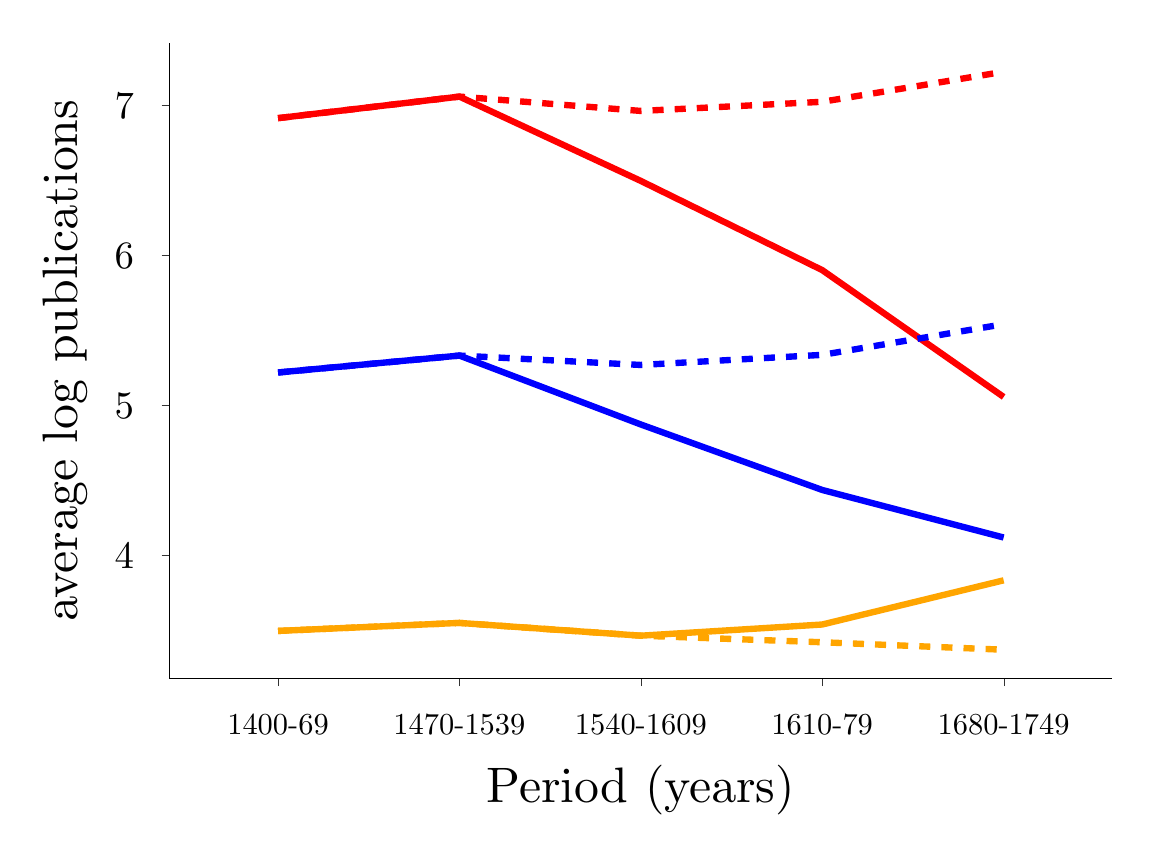
\begin{tikzpicture}[x=1pt,y=1pt]
\definecolor{fillColor}{RGB}{255,255,255}
\path[use as bounding box,fill=fillColor,fill opacity=0.00] (0,0) rectangle (397.48,289.08);
\begin{scope}
\path[clip] (  0.00,  0.00) rectangle (397.48,289.08);
\definecolor{drawColor}{RGB}{255,255,255}
\definecolor{fillColor}{RGB}{255,255,255}

\path[draw=drawColor,line width= 0.1pt,line join=round,line cap=round,fill=fillColor] (  0.00,  0.00) rectangle (397.48,289.08);
\end{scope}
\begin{scope}
\path[clip] ( 51.14, 53.86) rectangle (391.98,283.58);
\definecolor{fillColor}{RGB}{255,255,255}

\path[fill=fillColor] ( 51.14, 53.86) rectangle (391.98,283.58);
\definecolor{drawColor}{RGB}{255,0,0}

\path[draw=drawColor,line width= 2.3pt,line join=round] ( 90.47,256.38) --
	(156.02,264.17) --
	(221.56,233.70) --
	(287.11,201.47) --
	(352.66,155.64);

\path[draw=drawColor,line width= 2.3pt,dash pattern=on 4pt off 4pt ,line join=round] ( 90.47,256.38) --
	(156.02,264.17) --
	(221.56,258.99) --
	(287.11,262.29) --
	(352.66,273.14);
\definecolor{drawColor}{RGB}{0,0,255}

\path[draw=drawColor,line width= 2.3pt,line join=round] ( 90.47,164.47) --
	(156.02,170.59) --
	(221.56,145.69) --
	(287.11,122.03) --
	(352.66,104.85);

\path[draw=drawColor,line width= 2.3pt,dash pattern=on 4pt off 4pt ,line join=round] ( 90.47,164.47) --
	(156.02,170.59) --
	(221.56,167.20) --
	(287.11,170.85) --
	(352.66,181.93);
\definecolor{drawColor}{RGB}{255,165,0}

\path[draw=drawColor,line width= 2.3pt,line join=round] ( 90.47, 71.09) --
	(156.02, 73.99) --
	(221.56, 69.37) --
	(287.11, 73.41) --
	(352.66, 89.38);

\path[draw=drawColor,line width= 2.3pt,dash pattern=on 4pt off 4pt ,line join=round] ( 90.47, 71.09) --
	(156.02, 73.99) --
	(221.56, 69.37) --
	(287.11, 67.00) --
	(352.66, 64.30);
\end{scope}
\begin{scope}
\path[clip] (  0.00,  0.00) rectangle (397.48,289.08);
\definecolor{drawColor}{RGB}{0,0,0}

\path[draw=drawColor,line width= 0.1pt,line join=round] ( 51.14, 53.86) --
	( 51.14,283.58);
\end{scope}
\begin{scope}
\path[clip] (  0.00,  0.00) rectangle (397.48,289.08);
\definecolor{drawColor}{RGB}{0,0,0}

\node[text=drawColor,anchor=base east,inner sep=0pt, outer sep=0pt, scale=  1.40] at ( 38.39, 93.70) {4};

\node[text=drawColor,anchor=base east,inner sep=0pt, outer sep=0pt, scale=  1.40] at ( 38.39,147.89) {5};

\node[text=drawColor,anchor=base east,inner sep=0pt, outer sep=0pt, scale=  1.40] at ( 38.39,202.08) {6};

\node[text=drawColor,anchor=base east,inner sep=0pt, outer sep=0pt, scale=  1.40] at ( 38.39,256.27) {7};
\end{scope}
\begin{scope}
\path[clip] (  0.00,  0.00) rectangle (397.48,289.08);
\definecolor{drawColor}{gray}{0.20}

\path[draw=drawColor,line width= 0.1pt,line join=round] ( 48.39, 98.52) --
	( 51.14, 98.52);

\path[draw=drawColor,line width= 0.1pt,line join=round] ( 48.39,152.71) --
	( 51.14,152.71);

\path[draw=drawColor,line width= 0.1pt,line join=round] ( 48.39,206.90) --
	( 51.14,206.90);

\path[draw=drawColor,line width= 0.1pt,line join=round] ( 48.39,261.09) --
	( 51.14,261.09);
\end{scope}
\begin{scope}
\path[clip] (  0.00,  0.00) rectangle (397.48,289.08);
\definecolor{drawColor}{RGB}{0,0,0}

\path[draw=drawColor,line width= 0.1pt,line join=round] ( 51.14, 53.86) --
	(391.98, 53.86);
\end{scope}
\begin{scope}
\path[clip] (  0.00,  0.00) rectangle (397.48,289.08);
\definecolor{drawColor}{gray}{0.20}

\path[draw=drawColor,line width= 0.1pt,line join=round] ( 90.47, 51.11) --
	( 90.47, 53.86);

\path[draw=drawColor,line width= 0.1pt,line join=round] (156.02, 51.11) --
	(156.02, 53.86);

\path[draw=drawColor,line width= 0.1pt,line join=round] (221.56, 51.11) --
	(221.56, 53.86);

\path[draw=drawColor,line width= 0.1pt,line join=round] (287.11, 51.11) --
	(287.11, 53.86);

\path[draw=drawColor,line width= 0.1pt,line join=round] (352.66, 51.11) --
	(352.66, 53.86);
\end{scope}
\begin{scope}
\path[clip] (  0.00,  0.00) rectangle (397.48,289.08);
\definecolor{drawColor}{RGB}{0,0,0}

\node[text=drawColor,anchor=base,inner sep=0pt, outer sep=0pt, scale=  1.10] at ( 90.47, 33.53) {1400-69};

\node[text=drawColor,anchor=base,inner sep=0pt, outer sep=0pt, scale=  1.10] at (156.02, 33.53) {1470-1539};

\node[text=drawColor,anchor=base,inner sep=0pt, outer sep=0pt, scale=  1.10] at (221.56, 33.53) {1540-1609};

\node[text=drawColor,anchor=base,inner sep=0pt, outer sep=0pt, scale=  1.10] at (287.11, 33.53) {1610-79};

\node[text=drawColor,anchor=base,inner sep=0pt, outer sep=0pt, scale=  1.10] at (352.66, 33.53) {1680-1749};
\end{scope}
\begin{scope}
\path[clip] (  0.00,  0.00) rectangle (397.48,289.08);
\definecolor{drawColor}{RGB}{0,0,0}

\node[text=drawColor,anchor=base,inner sep=0pt, outer sep=0pt, scale=  1.80] at (221.56,  9.00) {Period (years)};
\end{scope}
\begin{scope}
\path[clip] (  0.00,  0.00) rectangle (397.48,289.08);
\definecolor{drawColor}{RGB}{0,0,0}

\node[text=drawColor,rotate= 90.00,anchor=base,inner sep=0pt, outer sep=0pt, scale=  1.80] at ( 17.90,168.72) {average log publications};
\end{scope}
\end{tikzpicture}
 }
  	\end{subfigure}
  	\caption{Baseline simulations (solid), simulations without cenosorship (dashed)}
  	\label{fig:exp}\vspace{0.5em}
  	\begin{minipage}{0.99\textwidth} % choose width suitably
  		{\footnotesize \textsc{Notes.} periods: 1:1400-70, 2:1470-1540, 3:1540-1610, 4:1610-80, 5:1680-1750. \par}
  	\end{minipage}
  \end{figure}
  
\end{frame}


\begin{frame}
	\frametitle{Results}
	From the counterfactual experiment we learn that\vspace{0.1cm}
	
	\begin{itemize}
	\item Censorship reduced by 27\% the average log publication per scholar in Italy in 1680-1750\vspace{0.2cm}
	\item  Half of this drop stems from the induced reallocation of talents towards compliant activities, while the other half arises from the direct effect of censorship on book availability.\vspace{0.5cm}
	\end{itemize}


\end{frame}

\begin{frame}
	\frametitle{Conclusion}
What we did:  \vspace{0.3cm}
	\begin{enumerate}
	\item Build a database of scholars' quality over the period 1400-1750 \vspace{0.3cm}
	\item Document two features of authors censorship over the period \vspace{0.3cm}
	\item Build a parsimonious model of knowledge diffusion and censorship and take it to the data
	\vspace{0.3cm}
	\item Run counterfactual experiment to asses the role of Church's censorship on the decline of knowledge production in early moder Italy
	\vspace{0.3cm}
	\item \textbf{Censorship reduced by 27\% the average log publication per scholar in Italy} 
\end{enumerate}
\vspace{0.6cm}
\end{frame}






\end{document}

